% Generated review copy; edit main.tex and sections.
\documentclass[11pt]{article}

\usepackage[margin=1in]{geometry}
\usepackage{amsmath,amssymb}
\usepackage{graphicx}
\usepackage{booktabs,array,tabularx,longtable}
\usepackage{xcolor}
\usepackage{pgfplots}
\pgfplotsset{compat=1.17}
\usetikzlibrary{positioning}
\usepgfplotslibrary{groupplots}
\usepgfplotslibrary{statistics}
\usepackage[hidelinks]{hyperref}
\urlstyle{same}

\newcolumntype{Y}{>{\raggedright\arraybackslash}X}
\newcommand{\pending}[1]{\par\smallskip\noindent
  \textit{Pending evidence. #1}\par\smallskip}
\newcommand{\SO}{\mathrm{SO}}
\newcommand{\R}{\mathbb{R}}

\title{Morphology-Conditioned Physics-Based Motion Imitation\\
Across 128 Body Shapes}
\author{}
\date{Connection Science working draft --- 10 October 2026}

% Compile from paper-draft/. October revision; pending GPU evidence is marked.

\begin{document}
\maketitle
\begin{abstract}
Learning one physics-based motion controller across bodies requires both
shared control and references consistent with each body's geometry. We study
this problem through three questions: shared tracking, unseen-body transfer,
and the design choices supporting them. A paired corpus links 20,951
HumanML3D clip identities to HUMOS references and matching simulated assets
for 128 body configurations. One morphology-conditioned temporal controller
trains on 18,855 clips across those bodies. It achieves 99.14\% tracking
success on 1,048 held-out motions, with one selected trained body per clip.
On 233 training-split clips replayed across each of two 128-body unseen
panels, success is 97.28\% inside the training coefficient range and 97.15\%
outside it. These averages coexist with individual-body success as low as
3.0\% and 13.3\%, respectively. A later checkpoint improves outside-panel
success but worsens inside-panel success, with substantial individual
regressions. Three-seed architecture comparisons reveal trade-offs between
tracking and smoothness; paired reference refinement reduces sliding and
penetration while increasing reference jerk. The evidence supports shared
learning and strong average transfer within the evaluated domain, while
leaving all-body held-out-motion coverage, the causal value of explicit
morphology inputs, and the mechanisms of severe failures unresolved.
\end{abstract}


\section{Introduction}\label{sec:introduction}
A shared physics-based controller must reproduce actions on bodies with
different proportions and dynamics. Changing limb lengths, collision
geometry, and mass distribution changes both the spatial realization of a
motion and the actuation needed to track it. The learning problem therefore
has two coupled axes: variation in motion and variation in body. Good
tracking on new motions for a familiar body does not establish transfer to
a new body, and a high average over bodies can conceal severe failures.

Large motion resources, shape-conditioned reference generation, and scalable
imitation provide the building blocks~\cite{amass,humanml3d,humos,phc,protomotions}.
Body-conditioned control is established~\cite{won2019}; PHC also supports
body variation, although its quantitative evaluations use the mean SMPL
body~\cite{phc}. Our question is how reliably one controller learns and
transfers across a large corpus of explicitly paired motions and bodies.
We address it through three research questions:
\begin{enumerate}
\item \textbf{RQ1: Can one shared controller learn to track diverse motions
across different bodies?} We distinguish held-out-motion performance on
selected bodies from coverage of every trained body.
\item \textbf{RQ2: How well does that capability generalise to unseen body
shapes, and where does it fail?} We evaluate inside- and outside-range bodies,
retain every shape, and examine checkpoint sensitivity.
\item \textbf{RQ3: Which design choices support that capability, and what
trade-offs do they introduce?} We compare temporal architectures and audit
reference refinement, while identifying the missing conditioning control.
\end{enumerate}

Our contribution is a paired corpus and learning workflow that preserves
clip/body identity from HUMOS generation through simulation and replay,
together with an evaluation that separates motion exposure from body
exposure. The corpus contains 20,951 clip identities and 128 body
configurations. A shared temporal slot/type-attention controller trains
directly on 18,855 clips across those bodies using streamed motion residency.
We inherit the simulator integration, PPO machinery, and motion-tracking
infrastructure from ProtoMotions; we do not claim these or morphology
conditioning itself as new. HumanML3D captions are metadata, not policy
inputs: this is reference-conditioned imitation, not text-conditioned control.

The original checkpoint achieves 99.14\% success on 1,048 independent test
clips, each paired with one selected trained body. On 233 training-split
clips across 128 unseen inside-range bodies and 128 unseen outside-range
bodies, success is 97.28\% and 97.15\%. Yet the worst bodies succeed on only
3.0\% and 13.3\% of those clips. These findings support the central claim:
\emph{one shared controller learns morphology-specific tracking with strong
average transfer to unseen shapes, but uneven robustness across individual
bodies}. The design evidence explains practical trade-offs; it does not yet
isolate the benefit of explicit morphology inputs or establish uniform
held-out-motion performance across all bodies.

\section{Related Work}\label{sec:related_work}

\subsection{Physics-based motion imitation}

DeepMimic demonstrated reference-guided reinforcement learning for simulated
character skills~\cite{deepmimic}. Perpetual Humanoid Control developed robust
humanoid imitation for real-time simulated avatars~\cite{phc}. These approaches
motivate learning a feedback controller rather than directly replaying a
kinematic trajectory. PULSE learns a motion representation for humanoid control, while OmniH2O,
ExBody2, and GMT study large-scale control on robot platforms~\cite{pulse,omnih2o,exbody2,gmt}.
ASE learns reusable latent skills and downstream task policies rather than
requiring exact clip tracking~\cite{ase}. These objectives provide context,
but their published scores do not measure our clip/body replay task.
We implement our experiments in ProtoMotions with Isaac Gym and PPO
optimization~\cite{protomotions,isaacgym,ppo}.

\subsection{Morphology-conditioned control and retargeting}

Body-shape variation has already been studied in physics-based control:
Won and Lee learned a parametric controller that accommodates variation in
character height, weight, and proportions~\cite{won2019}. A separate line of
work learns policies that transfer across changes in agent \emph{topology} --
limb count and skeletal structure -- through shared modular
sub-policies~\cite{smp2020}, which is a different axis from the continuous
anthropometric variation studied here. Morphology conditioning is therefore
an established idea, and our work should not be interpreted as introducing it.
We instead examine one controller over a large set of paired motions and
bodies, with shape identity maintained throughout data generation,
simulation, and evaluation.

Kinematic retargeting and dynamic tracking address different requirements.
SMPL provides a common parameterized body representation~\cite{smpl}, and
SMPLSim constructs simulation-ready assets from these
models~\cite{smplsim}. A shared skeleton makes poses comparable, but does not
make global positions or required actuation independent of shape. Matching a
reference to its intended simulation asset is consequently part of the task
definition, not an optional evaluation convenience.

\subsection{Text-motion data, shape-conditioned generation, and refinement}

AMASS consolidates motion capture in a common body-model
representation~\cite{amass}. HumanML3D associates processed motion segments
with natural-language descriptions~\cite{humanml3d}. We inherit those source
identities and descriptions rather than claiming new motion capture or
shape-specific language annotation.

HUMOS generates identity-conditioned human motion using a cycle-consistent
learning formulation~\cite{humos}. We use its pretrained model to obtain
shape-specific references, not as the physics controller and not as a
text-conditioned policy. The resulting sequences still require conversion to
the simulator's skeleton and coordinate conventions, and their feasibility
must be assessed in that simulator. Our refinement is a deliberately limited
kinematic post-process; it is not a new generative model or a full dynamic
trajectory optimizer.

The controller uses standard Transformer operations~\cite{attention}.
Learned slot and type embeddings identify temporal positions and observation
sources. An ablation also investigates actor-only morphology modulation with
adaLN-Zero, adapting the zero-initialized conditioning design used in
Diffusion Transformers~\cite{dit}. That experiment tests a conditioning
mechanism, not diffusion-based action generation.

\subsection{Headline capability and evidence comparison}
Table~\ref{tab:capabilities} separates published support from demonstrated
evaluation coverage. In particular, PHC's Appendix B describes shape-varying
humanoids and training with sampled AMASS shapes; its quantitative comparisons
use the mean neutral SMPL body~\cite{phc}. It is therefore inaccurate to
classify PHC as incapable of body variation. Won and Lee directly establish
parametric body control~\cite{won2019}. Our distinction is the paired corpus
and systematic inside/outside replay, not priority for morphology conditioning.

\begin{table}[p]
\centering\footnotesize
\caption{Published capabilities and evaluation scope, not a performance
ranking. ``Not reported'' concerns the cited source and the specified
unseen-body test, not impossibility. No external system has been rerun on our
matched references, assets, horizon, and aggregation. Software documentation
for ProtoMotions 3 is distinguished from paper evaluations and from the
implementation used in this study.}\label{tab:capabilities}
\begin{tabularx}{\linewidth}{@{}p{0.13\linewidth}YYY@{}}
\toprule
System / source & Task and motion evidence & Body capability & Evaluation relevance \\
\midrule
PHC~\cite{phc} & Reference tracking and recovery; 11,313 train and 140 test AMASS sequences. & SMPL shape/gender variation; sampled shapes and body-normalized references described. & Quantitative motion tests use mean neutral body; shape variation shown qualitatively. No systematic inside/outside unseen-body panel reported. \\[0.5em]
ASE~\cite{ase} & Latent skill pretraining and downstream tasks; 187 clips. Exact reference tracking is not its objective. & Published experiments use a sword/shield humanoid; a shared shape-conditioned body sweep is not reported. & Task transfer, skill coverage, and recovery evaluated; unseen-body clip-tracking test not reported. \\[0.5em]
ProtoMotions 3~\cite{protomotions} & Framework documents large-scale tracking, distributed training, retargeting, and generative policies. & Supports different configured characters/robots; this alone does not demonstrate one policy across shape variants. & Official README is a software capability source, not a matched multi-body benchmark. Our simulator/PPO/tracking infrastructure is inherited. \\[0.5em]
Won \& Lee~\cite{won2019} & Parametric physical character control with adaptive shape sampling. & One parametric controller accommodates height, weight, and proportion changes; new and changing bodies demonstrated. & Direct prior body-control capability; experiments differ from our large clip-by-body imitation panels. \\[0.5em]
HUMOS~\cite{humos} & Identity-conditioned motion generation with physical-consistency objectives. & Shape-conditioned motions; supplies our pretrained reference generator. & Not an online feedback tracker; its motion-generation scores are not tracking success under our simulator protocol. \\[0.5em]
This study & Shared tracking; 18,855 training identities, 1,048 held-out test identities. & 128 trained bodies; references and assets share identity. & Test: one trained body per clip. Unseen: 233 known clips $\times$ each of 128 inside and 128 outside bodies; all shapes retained. Conditioning mechanism remains unisolated. \\
\bottomrule
\end{tabularx}
\end{table}

\paragraph{Inherited functions and study additions.}
ProtoMotions provides the simulation abstraction, PPO training, motion-library
and imitation infrastructure. HUMOS supplies the pretrained generator;
SMPL/SMPLSim supply the body parameterization and asset construction. Our
study adds the paired corpus assembly and identity checks, reference
processing and fidelity audit, the evaluated temporal slot/type controller
configuration, streamed clip residency, and exposure-separated evaluation.
These are system and empirical contributions built on existing methods,
not claims to invent attention, PPO, body models, or motion imitation.
A directly comparable performance claim requires a matched external replay;
none is made here.

\section{Problem Formulation and System Overview}\label{sec:problem}
A body configuration $b=(g,\boldsymbol{\beta})$ specifies a SMPL template
and shape coefficients. For source clip $c$, HUMOS supplies a shape-specific
reference $\hat{s}_{c,b}(t)$ and SMPLSim supplies the matching asset. Changing
$b$ changes geometry, reference positions, mass/inertia, and mass-scaled
actuation even though topology is shared. The task is to track these paired
references with one policy, not impose identical world-space paths on all bodies.

We learn $\pi_\theta(a_t\mid o_t,b)$ using present state, history, future
reference targets, and body information. The same parameters serve every
body. Clips can change on reset while each environment retains its asset.
Evaluation preserves reference/body identity.

The system constructs paired references (Section~\ref{sec:dataset}), trains
a shared controller with streamed residency (Section~\ref{sec:method}), and
replays fixed pairs with known motion and morphology exposure
(Section~\ref{sec:experiments}). Figure~\ref{fig:data_pipeline} summarizes
the identity paths. Text is metadata, not a controller input. The flat-ground
task has no external objects or partners.

\section{Paired Motion and Body Corpus}\label{sec:dataset}

We construct a derived corpus in which a source clip identity connects a motion
description, 128 generated motion variants, and their matching simulation
assets. A \emph{clip} denotes a source segment, including a mirrored segment
when present; a \emph{variant} denotes that clip on one body configuration.
These units must not be conflated when reporting dataset size or evaluation
coverage. Figure~\ref{fig:data_pipeline} shows the construction paths and
Figure~\ref{fig:dataset_scale} the resulting scale and split structure.

\begin{figure}[t]
\centering
\fbox{\begin{minipage}{0.94\linewidth}
\small
\begin{tabularx}{\linewidth}{@{}p{0.12\linewidth}Y@{}}
\textbf{Motion} &
AMASS $\longrightarrow$ HumanML3D preprocessing and clip extraction
$\longrightarrow$ HUMOS conditioned on $(g,\boldsymbol{\beta})$
$\longrightarrow$ MotionLib conversion and reference refinement
$\longrightarrow$ per-clip motion variants. \\[0.7em]
\textbf{Body} &
SMPL with the same $(g,\boldsymbol{\beta})$
$\longrightarrow$ SMPLSim
$\longrightarrow$ matching skeleton, collision geometry, mass/inertia,
and MJCF asset identity. \\[0.7em]
\textbf{Text} &
HumanML3D source descriptions
$\longrightarrow$ clip-ID lookup associated with the generated variants
(metadata only; not a policy input).
\end{tabularx}

\smallskip
The body assets are used for motion conversion, shape-specific forward
kinematics, ground-clearance correction, and simulation. Refined reference
motion and matching simulated state feed one shared policy.
\end{minipage}}
\caption{Dataset and asset construction. The body parameters are shared across
the motion and body paths; text follows a separate identity-association path.}\label{fig:data_pipeline}
\end{figure}

\begin{figure}[t]
\centering
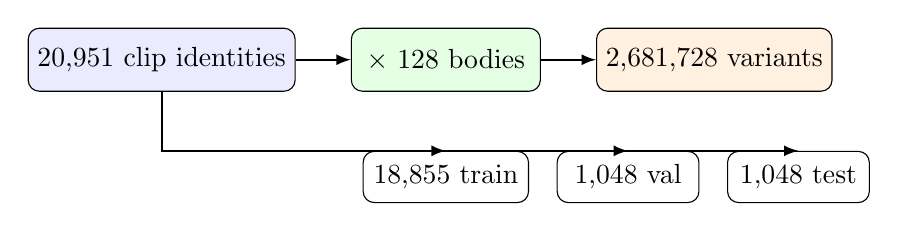
\begin{tikzpicture}[>=latex, node distance=0.7cm]
\node[draw, rounded corners, fill=blue!8, minimum width=2.4cm, minimum height=0.8cm]
  (source) {20,951 clip identities};
\node[draw, rounded corners, fill=green!10, right=of source, minimum width=2.4cm, minimum height=0.8cm]
  (variants) {$\times$ 128 bodies};
\node[draw, rounded corners, fill=orange!12, right=of variants, minimum width=2.4cm, minimum height=0.8cm]
  (total) {2,681,728 variants};
\draw[->, thick] (source) -- (variants);
\draw[->, thick] (variants) -- (total);
\node[draw, rounded corners, below=0.75cm of variants, minimum width=2.1cm, minimum height=0.65cm]
  (train) {18,855 train};
\node[draw, rounded corners, right=0.35cm of train, minimum width=1.8cm, minimum height=0.65cm]
  (val) {1,048 val};
\node[draw, rounded corners, right=0.35cm of val, minimum width=1.8cm, minimum height=0.65cm]
  (test) {1,048 test};
\draw[->, thick] (source.south) |- (train.north);
\draw[->, thick] (source.south) |- (val.north);
\draw[->, thick] (source.south) |- (test.north);
\end{tikzpicture}
\caption{Scale and split structure of the derived corpus. Splitting is by clip
identity, so all 128 body variants of a clip remain in the same partition.}
\label{fig:dataset_scale}
\end{figure}

\subsection{Source motion and text provenance}\label{sec:source_data}

We use the AMASS-derived motion portion of HumanML3D~\cite{amass,humanml3d}, with the 18 source collections listed in
Appendix~\ref{app:preprocessing}. Source SMPL+H sequences are processed at
20\,Hz, including the Z-up to Y-up coordinate conversion used by the
HumanML3D/HUMOS preprocessing pipeline. Clip extraction, temporal cropping, and
mirroring preserve the HumanML3D identities. The preparation also includes
treadmill/skating cleanup. This subset is not the entirety of AMASS.

The generation pipeline produced 22,459 candidate clip identities, counting
original and mirrored clips. A subsequent text-based filter excluded 1,508
clips identified as requiring external objects or environmental support,
leaving 20,951 identities for the flat-ground imitation task. This filter is a
task-scope heuristic: it does not prove that every retained reference is
support-free or dynamically feasible. The retained and excluded ID lists
provide the audit trail for that decision.

Source descriptions are available through a separate clip-ID lookup and the
HumanML3D annotation metadata used by HUMOS. A description is associated with
the variants of its source clip; it is not a new human annotation for each
generated body. A coarse coverage check against a single-caption-per-clip
lookup finds a caption for all 20,951 clip identities, but semantic fidelity
is not established. Of the 9,579 mirrored identities, 22\% carry a caption
byte-identical to their un-mirrored source, and 40\% contain an explicit
left/right or clockwise term that mirroring inverts; simply removing a mirror
prefix therefore does not establish a correct caption. Segment timing and
multi-annotation coverage against the full HumanML3D annotation set are not
audited here.

\subsection{Body sampling and shape-specific generation}\label{sec:body_generation}

Let a body configuration be $b=(g,\boldsymbol{\beta})$, where $g$ identifies the
female or male SMPL body-model variant and
$\boldsymbol{\beta}\in\R^{10}$ contains shape coefficients. We sample
\begin{equation}
    \beta_{ij}\sim\mathcal{U}(-3,3),\qquad
    i=1,\ldots,64,\quad j=1,\ldots,10,
    \label{eq:shape_sampling}
\end{equation}
using NumPy's \texttt{default\_rng(46)}, and cross these 64 vectors with the two
body-model variants. Thus the corpus contains 128 body configurations, not
128 independently sampled beta vectors. The actual coefficient arrays and
stable beta keys identify the bodies; the keys are not content hashes.
Uniform sampling of model coefficients is a controlled source of variation,
not a representative sample of human populations.

For each source clip, we provide the processed pose/root motion features and
the target body parameters to the pretrained HUMOS
model~\cite{humos}. The local configuration uses root-relative 6D root and
joint rotations together with translation, with shape and body-model
conditioning. The generated pose and root sequences are retained for
conversion. HUMOS is an existing identity-conditioned model; neither its
training nor a text-to-motion generator is a contribution of this work.
The checkpoint used in the documented pipeline is identified in
Appendix~\ref{app:provenance}.

In parallel, SMPL bodies~\cite{smpl} with identical parameters are converted
to MJCF assets using SMPLSim~\cite{smplsim}. The asset-generation configuration
uses mass estimation and the configured hand/foot simplifications
(\texttt{real\_weight}, \texttt{replace\_feet}, \texttt{remove\_toe}, and
\texttt{freeze\_hand}). The resulting imitation representation contains
24 rigid bodies and 69 actuated joint coordinates. Collision proxies, joint
ranges, and estimated masses/inertias belong to each asset. These physical
parameters are simulation-model estimates, not measurements of corresponding
human participants.

\subsection{Motion conversion and reference refinement}\label{sec:refinement}

The generated sequences are converted to ProtoMotions' Z-up simulation
convention and resampled from 20 to 30\,Hz. Forward kinematics (FK) uses the
matching asset rather than a single neutral skeleton. The packaged
representation includes global body positions and rotations, local rotations,
joint positions, linear/angular and joint velocities, and contact labels.
The earlier corpus already included frame-zero grounding; the newer
refinement addresses artifacts throughout each sequence.

Refinement is applied independently to each variant in the following order.
First, stored ankle/toe contacts are validated, or contacts are detected from
foot position and velocity if usable labels are unavailable. Short gaps are
closed and very short contact runs are removed. These labels define candidate
stance intervals; they are not measured ground-reaction forces.

Second, joint rotations are temporally filtered using sign-continuous
quaternion representations, normalization, and a bounded geodesic correction.
Contact-transition frames divide the sequence into segments so filtering does
not average across a change of stance. A transition taper and a limited
smoothing blend further restrict changes near those boundaries.
Post-smoothing FK then recomputes the positions used by subsequent corrections.

Third, a conservative root-translation correction reduces horizontal stance
sliding. For each contact interval, an anchor is formed from the foot's median
horizontal position. A least-squares correction seeks a common root XY shift
that brings the active feet closer to their anchors; the shift is temporally
regularized and capped. Multiple contacts can disagree, so this root-only
operation does not guarantee exact foot locking and does not solve for new
joint angles.

Fourth, we evaluate the lowest point of the matching collision geometry at
every frame. With floor height zero and margin $\epsilon_z$, the required lift is
\begin{equation}
    \ell_t^{\mathrm{req}}
      = \max\!\left(0,\epsilon_z-\min_{x\in\mathcal{C}_b(t)}x_z\right),
    \label{eq:clearance}
\end{equation}
where $\mathcal{C}_b(t)$ denotes the modeled collision geometry for body $b$.
A smoothed lift envelope is constrained to remain above this requirement.
This prevents penetration of the checked geometry in the reference sequence;
it does not establish balanced support, realistic impacts, or freedom from
self-collision.

Finally, FK and velocities are recomputed from the corrected root and
rotations, independently within each motion. This avoids inconsistent
position/velocity tensors and artificial derivatives across clip boundaries.
The default thresholds, filter windows, and correction bounds are given in
Table~\ref{tab:refinement_parameters}.

The refinement objective is modest: reduce visible and measurable kinematic
artifacts while preserving the generated motion. Before/after assessment must
therefore include both artifact measures (sliding, penetration, and jerk) and
fidelity measures (rotation/root changes and retained cross-shape variation).
Improved kinematics alone does not demonstrate improved policy learning or
dynamic feasibility.

\subsection{Packaging, scale, and deterministic splits}\label{sec:splits}

Each per-clip file contains the 128 variants, their frame counts and sampling
rates, and the clip/asset identities needed to recover the corresponding body
parameters. Captions remain a separately associated metadata resource; they
are not established as a field of every training tensor file. This packaging
allows the training system to stream clip files without downloading the
complete corpus at startup.

\begin{table}[t]
\centering
\caption{Current corpus and split sizes. Variants are generated combinations,
not independent captures. Every clip has 128 body configurations.}\label{tab:dataset_counts}
\begin{tabular}{lrr}
\toprule
Partition & Clip identities & Motion variants \\
\midrule
Training & 18,855 & 2,413,440 \\
Validation & 1,048 & 134,144 \\
Test & 1,048 & 134,144 \\
\midrule
Total & 20,951 & 2,681,728 \\
\bottomrule
\end{tabular}
\end{table}

We use the versioned \texttt{hhi\_stage2\_v1} split with seed 42 and approximate
90/5/5 proportions (Table~\ref{tab:dataset_counts}). All variants of a clip
stay together, and original/mirrored partners are assigned as a group.
The 150 development clips are reserved for training, together with their
mirror partners. Training accepts explicit training and validation manifests;
test-manifest membership is not loaded by the training workflow. Split hashes
and version information accompany the run and checkpoints.

These splits test held-out clip identities on the trained body set. They have
not been demonstrated to be disjoint by subject or original capture recording:
different segments can still share a source recording. This distinction
limits claims about broader motion generalization.

\subsection{Current resource scope}

The current resource combines generated references, matching assets, inherited
text associations, and reproducible splits. It is not a fully audited
text-and-motion benchmark release. Caption completeness and alignment,
body-specific language, licensing and redistribution conditions, and
shape-conditioned semantic fidelity require further work. Those extensions
can be developed independently of the reference-conditioned controller
evaluated here.

\section{Shared Controller and Training}\label{sec:method}

\subsection{Task, simulation, and actuation}

The policy follows the task in Section~\ref{sec:problem}.

Experiments use the \texttt{smpl\_mor} assets in Isaac Gym through
ProtoMotions~\cite{isaacgym,protomotions}. Simulation runs at 60\,Hz with two
substeps and control decimation two, giving a 30\,Hz policy rate. The policy
outputs a raw action $a_t\in\R^D$, where $D=69$. Joint targets are
\begin{equation}
    q_t^{\mathrm{target}}
      = q^{\mathrm{offset}}
        + q^{\mathrm{scale}}\odot\tanh(a_t),
    \label{eq:action_mapping}
\end{equation}
with offsets and scales derived from the configured joint ranges. These
targets drive the simulator's built-in position PD controller. The action is
not a residual added to the reference pose.

PD stiffness, damping, and effort limits are scaled per joint by the mass of
its associated rigid body relative to that body in the reference asset.
This is a body-level mass scaling, not a single scale based on total character
mass, and it does not guarantee dynamically equivalent actuation across
geometrically different bodies. Base gains and limits are listed in
Table~\ref{tab:pd_parameters}.

\subsection{Observation design}\label{sec:observations}

The observation combines present state, history, future reference targets,
a historical action, and explicit morphology information.
Let $B=24$ denote the number of simulated bodies. The state representation
contains root height above ground, root-relative body positions excluding
the root, 6D body rotations, and linear/angular velocities.
Positions and velocities use a heading-aligned frame, and rotations remove
the root heading. This removes dependence on arbitrary global heading and
horizontal origin while retaining height and body configuration.

We include seven historical states at control-step offsets
$\{1,2,3,4,8,16,32\}$, covering approximately 1.07\,s, and four future
reference slots at $\{1,2,4,8\}$, covering approximately 0.27\,s.
Each historical state uses its own root/heading frame.
Future slots contain target positions relative to the current root,
heading-aligned target rotations, position differences from the current body
state, relative rotations $\smash{R_{t,j}^{-1}\hat{R}_{t+k,j}}$, and
heading-aligned linear/angular velocity differences. Thus relative rotations
are expressed with respect to the current body rotation, not as another
heading-frame position feature.

\begin{table}[t]
\centering
\small
\caption{Observation inputs supplied to both actor and critic. Dimensions are
per slot. Positions/heights use meters, linear velocities m/s, angular
velocities rad/s, and 6D rotations are dimensionless. Raw actions and
morphology coefficients are not joint-angle measurements.}\label{tab:observations}
\begin{tabularx}{\linewidth}{@{}lrlY@{}}
\toprule
Input & Dimension & Slots & Representation and path \\
\midrule
Current state & $15B-2=358$ & 1 &
Height; $3(B-1)$ positions; $6B$ rotations; $3B$ linear and $3B$ angular
velocities. Current-state encoder. \\
History & $358$ & 7 &
Same state representation at the seven past offsets. Shared history encoder. \\
Future reference & $24B=576$ & 4 &
Target and relative poses ($18B$), plus velocity differences ($6B$).
Shared future encoder. \\
Historical action & $D=69$ & 1 &
A raw previous policy-action vector, before tanh and PD scaling.
Bypasses attention. \\
Morphology & $11$ & 1 &
$[g,\beta_1,\ldots,\beta_{10}]$ from the assigned asset.
Bypasses attention. \\
\bottomrule
\end{tabularx}
\end{table}

The temporal context exposes both recent changes and more distant motion
information; the future targets provide a short anticipation window.
These are design motivations, not established ablation outcomes.
History is initialized consistently with reference-state resets using
available historical reference states; single-state initialization is the
fallback when a trajectory history is unavailable.
Contact flags, an explicit phase scalar, text, and estimated physical
feature vectors are not part of the selected observation.

\subsection{Temporal slot/type attention}\label{sec:architecture}

We use three observation encoders: one for the current state, one shared
across history slots, and one shared across future slots. Each is an MLP
with two 256-unit ReLU hidden layers and a 256-dimensional token output.
Inputs use running mean/standard-deviation normalization and a magnitude
clamp of five.

The resulting 12 tokens comprise one current, seven historical, and four
future tokens. For slot $i$, the Transformer input is
\begin{equation}
    z_i = E_{\tau(i)}(x_i)
        + e_i^{\mathrm{slot}} + e_{\tau(i)}^{\mathrm{type}},
    \qquad i=0,\ldots,11,
    \label{eq:token_embedding}
\end{equation}
where $\tau(i)$ identifies the current/history/future source.
Slot embeddings distinguish the configured temporal offsets, while type
embeddings distinguish the observation sources. The Transformer has two
layers, four attention heads, token width 256, and feed-forward width
1,024~\cite{attention}. Its current-state token supplies the pooled output
after the configured output projection and activation.

\begin{figure}[t]
\centering
\fbox{\begin{minipage}{0.94\linewidth}
\small
\begin{tabularx}{\linewidth}{@{}YcY@{}}
Current state: $1\times358$ & $\longrightarrow$ &
Current encoder: $1\times256$ token \\
Past states: $7\times358$ & $\longrightarrow$ &
History encoder: $7\times256$ tokens \\
Future targets: $4\times576$ & $\longrightarrow$ &
Future encoder: $4\times256$ tokens
\end{tabularx}
\begin{center}
$\downarrow$\\
12 tokens + learned temporal-slot and source-type embeddings\\
$\downarrow$\\
2 Transformer layers, 4 heads, width 256\\
$\downarrow$\\
Pool current token: $h_t\in\R^{256}$\\
$\downarrow$\\
Concatenate $[h_t,\ a^{\mathrm{hist}}_t,\ g,\boldsymbol{\beta}]$
and normalize
\end{center}
\begin{tabularx}{\linewidth}{@{}YY@{}}
\textbf{Actor:} six 2,896-unit layers
$\longrightarrow$ 69 action means
$\longrightarrow$ tanh/range scaling
$\longrightarrow$ PD targets. &
\textbf{Critic:} four 1,024-unit layers
$\longrightarrow$ scalar state value.
\end{tabularx}
\smallskip
The entire encoder/attention pathway is instantiated separately for actor
and critic; the drawing summarizes the common design, not shared weights.
Morphology and action bypass attention into each head. Text is absent.
\end{minipage}}
\caption{Observation-to-action data flow of the selected slot/type policy.
Both networks receive the same input categories but have separate parameters.}\label{fig:network}
\end{figure}

The final head input is the concatenation of the 256-dimensional attention
output, the historical raw action, and the 11-dimensional morphology vector.
This 336-dimensional input also uses running normalization and clamp five.
Betas are not manually divided by three, embedded as a separate attention
token, or used for adaLN modulation in the selected model.

Actor and critic have separate token encoders, attention modules, slot/type
embeddings, and MLP heads. The actor head has six hidden layers of width
2,896; the critic has four of width 1,024, all with ReLU activations.
The outputs are a Gaussian action mean and a scalar value, respectively.
PPO samples actions with fixed diagonal log standard deviation $-2.9$;
evaluation uses the mean action. Figure~\ref{fig:network} summarizes the flow.

\subsection{Tracking reward, resets, and PPO}\label{sec:learning}

The training reward combines global body tracking and root-height tracking.
For corresponding simulated and reference body positions $p_j,\hat{p}_j$,
rotations $R_j,\hat{R}_j$, and velocities $v_j,\hat{v}_j$ and
$\omega_j,\hat{\omega}_j$, define
\begin{align}
    e_p &= \frac{1}{3B}\sum_{j=1}^{B}\|p_j-\hat{p}_j\|_2^2,
    & e_R &= \frac{1}{B}\sum_{j=1}^{B}
                  d_{\SO(3)}(R_j,\hat{R}_j)^2, \\
    e_v &= \frac{1}{3B}\sum_{j=1}^{B}\|v_j-\hat{v}_j\|_2^2,
    & e_\omega &= \frac{1}{3B}\sum_{j=1}^{B}
                     \|\omega_j-\hat{\omega}_j\|_2^2, \\
    e_h &= (h-\hat{h})^2, &&
\end{align}
where $d_{\SO(3)}$ is the geodesic rotation angle in radians.
The coordinate-wise means in the position and velocity errors match the
implemented reductions. The reward is
\begin{equation}
\begin{split}
    r_t ={}& 0.5\exp(-25e_p) + 0.3\exp(-5e_R)
             + 0.1\exp(-0.5e_v)\\
           &+0.2\exp(-0.1e_\omega) + 0.2\exp(-100e_h).
\end{split}\label{eq:reward}
\end{equation}
The weights are not normalized to sum to one. There is no explicit effort,
action-smoothness, or contact-matching reward in this experiment, and there
is no source-dependent switch between canonical and HUMOS reward functions.

References are sampled only from variants matching the environment's asset.
Reference-state initialization starts at frame zero with probability 0.2;
otherwise it uses a random valid reference time. Training episodes have a
maximum of 1,000 control steps and use the configured fall termination with
a 0.15\,m height setting and permitted foot-contact bodies. Tracking-error
termination is disabled. This training rule is distinct from the evaluation
failure threshold in Section~\ref{sec:metrics}.

We optimize using PPO~\cite{ppo}, with 32-step rollouts, discount 0.99,
GAE parameter 0.95, policy-ratio clipping 0.2, and normalized advantages.
Separate Adam optimizers use learning rates $2\times10^{-5}$ for the actor
and $10^{-4}$ for the critic. Other configuration values and actual run
budgets appear in Table~\ref{tab:training_parameters}. Evaluation rollouts
use deterministic inference without gradient tracking.

\subsection{Direct multi-shape learning and streamed sampling}\label{sec:sampling}

The final approach is direct multi-shape training on refined HUMOS
references. A small static corpus supports initial development; the
full-scale experiment streams per-clip files through \texttt{GlobalClipPool}.
The training manifest is deterministically partitioned across GPU ranks.
Each rank maintains a bounded resident pool containing all 128 variants
of its selected clips. Environment-level motion sampling respects the
assigned morphology.

At each scheduled rebuild, most resident slots are selected by explicit
top priority, combining estimated clip difficulty and an exploration bonus.
A fraction 0.2 is reserved for uniform random selection, maintaining rehearsal
outside the highest-priority set. Difficulty estimates are updated from
training-pool evaluations with an exponential moving average of rate 0.1
and a floor of 0.05. The exploration coefficient is 1.0.
This is a training curriculum, not uniform sampling of the complete corpus.

The resident pool is rebuilt every 256 epochs. The full-scale run initially
used 256 clips per rank and was resumed with 128 after memory failures; the
local cache multiplier was reduced to 1.0. These changes affect residency
and memory demand, not the underlying training split. Validation membership
is fixed independently of pool rebuilding, and validation evaluation does
not update training sampling weights. We report resident-pool and validation
metrics separately because they measure different populations.

\section{Evaluation Protocol}\label{sec:experiments}

\subsection{Development subset and full-scale protocol}

The development corpus contains 150 clips and all 128 body configurations,
for 19,200 variants. These clips are reserved within the full training split
and are not a held-out generalization benchmark. Small-scale experiments
investigate architecture and reference-processing choices with a fixed
simulation budget. The full-scale run uses the 18,855 training clips in
Table~\ref{tab:dataset_counts}, with validation membership fixed throughout.

The selected full-scale experiment is slot/type attention trained directly on
refined references. Its code retains a historical \texttt{stage2} name, but
this run does not use neutral pretraining followed by shape transfer.
Table~\ref{tab:training_parameters} records the shared optimization settings
and the actual environment/batch sizes used after the initial memory-related
launch adjustments. Run-specific resolved configurations take precedence
over older launch examples.

\begin{table}[t]
\centering
\small
\caption{Training configuration and budgets. Environment and minibatch counts
are per GPU. The full-scale frame count is a recorded stopping snapshot,
not a budget matched to the development runs.}\label{tab:training_parameters}
\begin{tabularx}{\linewidth}{@{}lYY@{}}
\toprule
Setting & Corrected 150-clip runs & Full-scale selected run \\
\midrule
Parallel GPUs per policy & 1 & 6 \\
Environments per GPU & 4,096 & 2,048 \\
PPO minibatch size per GPU & 16,384 & 8,192 \\
Rollout length & 32 control steps & 32 control steps \\
Mini-epochs per update & 1 & 1 \\
Actor / critic learning rates &
$2\times10^{-5}$ / $10^{-4}$ & $2\times10^{-5}$ / $10^{-4}$ \\
Discount / GAE / ratio clip & 0.99 / 0.95 / 0.2 & 0.99 / 0.95 / 0.2 \\
Gradient norm clip & 50 & 50 \\
Evaluation cadence & 200 epochs & 256 epochs \\
Training seed & 0--2 (refined A--D); 0 (unrefined E--H) & Recorded in saved run configuration \\
Reference residency & All 150 clips & 256, later 128 clips per GPU \\
Training frames & 786,432,000 per run (6,000 epochs) & Approximately $11.07\times10^9$ recorded \\
Status of reported evidence & Completed, Table~\ref{tab:architecture_seeds} & Epoch-28,170 checkpoint, Table~\ref{tab:test_results} \\
\bottomrule
\end{tabularx}
\end{table}

\subsection{Design comparisons and aggregation}\label{sec:ablation_design}
We compare four architectures: A, temporal MLP; B, temporal attention; C,
attention with slot/type embeddings; and D, C with actor-only adaLN-Zero.
All retain morphology inputs in actor and critic. Refined-reference runs
use three seeds (0, 1, 2), a matched 6,000-epoch budget, and the same cadence.
Each run is summarized by its last eight evaluations (epochs 4,600--6,000);
architecture means and sample standard deviations are then computed across
three run summaries. Within-run evaluations are not training replicates.

The full-scale model predates these supporting reruns. They reassess its
design rather than establish prospective selection or statistical superiority.
Models differ in parameter count; compute details are in Appendix~\ref{app:history}.
The original seed-0 grid is retained in Table~\ref{tab:ablation_results}.
Unrefined cases E--H have one seed each. Refined and unrefined policies track
their own targets, preventing a causal policy-level refinement conclusion.
The paired offline reference audit provides the evidence for artifact reduction.
\begin{table}[t]
\centering
\small
\caption{Corrected 150-clip grid: four architectures $\times$ two reference
versions, seed 0. Refined A--D also have seed-1/2 repeats in Table~\ref{tab:architecture_seeds}.}\label{tab:ablations}
\begin{tabularx}{\linewidth}{@{}llYY@{}}
\toprule
Case & References & Architecture & Comparison purpose \\
\midrule
A & Refined & Wide temporal MLP; beta concatenation &
Temporal MLP baseline. \\
B & Refined & Basic temporal attention &
Attention versus flattened temporal input. \\
C & Refined & Attention with slot/type embeddings &
Explicit temporal/source identity. \\
D & Refined & C + actor-only adaLN-Zero &
Morphology modulation with critic unchanged. \\
E & Unrefined & As C &
Reference version at fixed architecture (slot/type). \\
F & Unrefined & As A &
Reference version at fixed architecture (temporal MLP). \\
G & Unrefined & As B &
Reference version at fixed architecture (attention). \\
H & Unrefined & As D &
Reference version at fixed architecture (slot/type + adaLN). \\
\bottomrule
\end{tabularx}
\end{table}
\subsection{Morphology-matched evaluation and checkpoint scope}\label{sec:evaluation_protocol}

Each reference is rolled out only in an environment using its exact asset
identity (Figure~\ref{fig:evaluation_protocol}). A selected reference
therefore cannot be assigned to a different body simply because an
environment slot is available. Multiple rollout batches may be needed when
several references require the same body.

Routine monitoring selects one variant per clip. With seed $s=42$, stable
clip identity $c$, panel index $p$, and $N_c$ available variants, the choice is
\begin{equation}
    k(c,p) =
    \left(
       \operatorname{uint64}_{\mathrm{big}}
       \bigl(\operatorname{SHA256}(s\!:\!c)_{0:8}\bigr)
       +p
    \right)\bmod N_c .
    \label{eq:shape_panel}
\end{equation}
Here $s\!:\!c$ is the UTF-8 string formed as \texttt{seed:clip\_id}.
For scheduled monitoring, $p$ is the integer quotient of the checkpointed
epoch and evaluation cadence. This produces deterministic staggered shape
choices that rotate across evaluations and remain reproducible after resume.
The validation \emph{clip list} is fixed; the selected \emph{shape panel}
changes. Thus successive scores are not repeated measurements on an
identical set of clip/shape pairs.

Evaluation uses the mean action, reference initialization, and no gradient
tracking. It disables training termination and records errors over the
valid reference horizon, capped at 600 control steps (20\,s at 30\,Hz).
Success therefore refers to the evaluated horizon, not necessarily the
entire duration of a longer source clip.

Final model comparisons should freeze the checkpoint, clip/shape panel,
reference version, simulator configuration, and seed. Validation is available
for model selection and has been repeatedly monitored; it is not an untouched
test set. The independent test manifest remains outside training and model
selection; its one-time evaluation is reported in
Section~\ref{sec:test_results}. The downloaded epoch-28,170
\texttt{last.ckpt} is distinct from the epoch-28,159 monitoring snapshot
in Table~\ref{tab:full_results}; the standalone validation and test results
therefore refer explicitly to the downloaded checkpoint.

\begin{figure}[t]
\centering
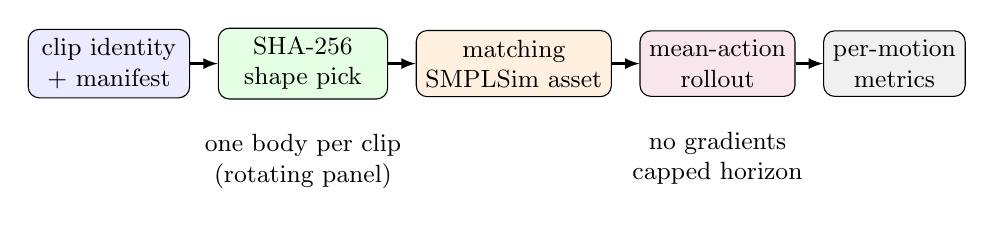
\begin{tikzpicture}[>=latex, node distance=0.35cm, every node/.style={font=\small}]
\node[draw, rounded corners, fill=blue!8, align=center, minimum width=2.05cm, minimum height=0.72cm] (clip) {clip identity\\+ manifest};
\node[draw, rounded corners, fill=green!10, right=of clip, align=center, minimum width=2.15cm, minimum height=0.72cm] (pick) {SHA-256\\shape pick};
\node[draw, rounded corners, fill=orange!12, right=of pick, align=center, minimum width=2.15cm, minimum height=0.72cm] (asset) {matching\\SMPLSim asset};
\node[draw, rounded corners, fill=purple!10, right=of asset, align=center, minimum width=1.9cm, minimum height=0.72cm] (roll) {mean-action\\rollout};
\node[draw, rounded corners, fill=gray!12, right=of roll, align=center, minimum width=1.75cm, minimum height=0.72cm] (metrics) {per-motion\\metrics};
\draw[->, thick] (clip) -- (pick);
\draw[->, thick] (pick) -- (asset);
\draw[->, thick] (asset) -- (roll);
\draw[->, thick] (roll) -- (metrics);
\node[below=0.32cm of pick, align=center] {one body per clip\\(rotating panel)};
\node[below=0.32cm of roll, align=center] {no gradients\\capped horizon};
\end{tikzpicture}
\caption{Standalone evaluation protocol. The clip list is fixed, while a
reproducible hash-and-panel rule selects one body variant per clip; the
selected reference and simulation asset therefore always match.}
\label{fig:evaluation_protocol}
\end{figure}

\subsection{Metrics and aggregation}\label{sec:metrics}

For each evaluated clip/shape pair $i$, define its per-frame mean body
position error
\begin{equation}
    d_{i,t} = \frac{1}{B}\sum_{j=1}^{B}
                 \|p_{i,t,j}-\hat{p}_{i,t,j}\|_2 .
\end{equation}
The configured success indicator is
\begin{equation}
    S_i = \mathbf{1}\!\left[
             \max_{t<T_i}d_{i,t}\leq 0.5\ \mathrm{m}
          \right],
    \label{eq:success}
\end{equation}
where $T_i$ is the evaluated horizon. This threshold is deliberately distinct
from the smoother training reward. Passing it does not imply fine-grained
pose accuracy or biomechanical realism.

We also report time-averaged mean body-position error, mean global
body-rotation geodesic error, and the time average of the largest body-position
error within each frame. The last quantity is the logged
\emph{mean maximum-joint error}; it is not the maximum over the entire dataset.
Global body-rotation error is not a local joint-angle/DOF error.

Within an evaluator rank, errors are averaged over valid frames per motion
and then over motions, including failed rollouts. The distributed training
logger aggregates scalar summaries across ranks; the monitoring table
retains those logged values rather than reconstructing exact pooled counts.
Final offline comparisons should aggregate saved per-motion records over
unique clip/shape pairs, avoiding unequal weighting of partially filled
batches or duplicate padded rollouts.

Trajectory smoothness uses the implementation's windowed normalized-jerk
score, with the definition and numerical regularizers in
Appendix~\ref{app:smoothness}. Lower scores indicate lower jerk under that
fixed convention. The accompanying high-jerk statistic is the percentage
of windows in which any body exceeds threshold 6,500; the logger calls it
a frame percentage, but it is window-based.


\subsection{Research questions, populations, and checkpoint scope}
Table~\ref{tab:evidence_populations} maps the evidence to the three questions.
Held-out identity is clip-grouped, not a demonstrated subject/recording split.
\begin{table}[t]
\centering\small
\caption{Evaluation populations and their inference scope. Each unseen panel
has 128 bodies; the 233-clip and 23-clip subsets partition its 256 clips.}
\label{tab:evidence_populations}
\begin{tabularx}{\linewidth}{@{}lYYr@{}}
\toprule
Question & Motion exposure & Body exposure & Pairs \\
\midrule
RQ1: validation / test & Held-out clips & Trained; one per clip & 1,048 each \\
RQ1: development replay & 150 training clips & All 128 trained & 19,200 \\
RQ2: inside / outside & 233 training clips & All 128 unseen per panel & 29,824 each \\
RQ2: diagnostic subset & 23 val/test clips; seen by full-data & Same unseen panels & 2,944 each \\
RQ2: trained control & 150 training clips & All 128 trained & 19,200 \\
RQ3: design comparison & Development clips & Trained bodies & Three refined seeds \\
\bottomrule
\end{tabularx}
\end{table}

\paragraph{Unseen-body construction and replay.}
Each panel contains 64 new coefficient vectors instantiated on male and female
SMPL templates. Inside vectors lie in $[-3,3]^{10}$; outside vectors have
$\|\beta\|_\infty\in(3,5]$, with 16 vectors (32 bodies) in each of four
half-unit tiers. Inside denotes membership of the training coefficient box,
not demonstrated membership of the convex hull of trained bodies. Both
panels use matching HUMOS references and assets, frame-zero offsets and
full reference refinement. The build report records finite complete clip/body
panels and zero penetration under its refinement diagnostic; it does not
certify dynamic feasibility.

All nine runs completed on an A40 on 9 October 2026. Replay uses mean actions,
reference initialization, 32 environments per asset (4,096 environments),
and at most 210 control steps (7\,s). Success follows Eq.~\eqref{eq:success}.
The 233 training-split identities isolate the body axis; the other 23
validation/test identities remain separate. The trained-body control uses a
different 150-clip panel and refinement run, so only within-dataset checkpoint
deltas are paired comparisons.

\paragraph{Checkpoint and uncertainty controls.}
The original \texttt{refined} checkpoint is epoch 28,170; the prespecified
\texttt{fulldata} candidate is epoch 34,000 and trained on all original motion
splits. Both are frozen for replay. Duration and motion coverage change
together, preventing causal attribution. Each dataset has two original-checkpoint
runs and one candidate run. Paired 95\% bootstrap intervals resample clips,
retaining the full fixed body panel; they do not resample training seeds or
unseen bodies. The report's ``beyond noise'' rule requires an interval excluding
zero and a candidate delta larger in magnitude than the original-checkpoint
rerun delta. With no checkpoint ladder, that comparison measures simulator
variability only. Per-body regression intervals are exploratory and unadjusted
for multiple testing.

On all 256 clips, identical-checkpoint success labels agree on 99.33\% of
inside and 98.68\% of outside pairs, versus 99.96\% in the control. Pooled
success differs by at most 0.05 pp, but individual pairs can change by metres
in peak error. Small pooled changes therefore coexist with local instability.
Checkpoint hashes and the retained report are documented in
Appendix~\ref{app:provenance}; complete per-body tables are in
Appendix~\ref{app:unseen_tables}.

\section{Results}\label{sec:results}
We assess held-out tracking, distinguish trained-body coverage from unseen
transfer, and use design comparisons and failures to delimit the claim.

\subsection{RQ1: Shared tracking across motions and bodies}\subsubsection{Held-out motions on selected trained bodies}\label{sec:test_results}

The epoch-28,170 checkpoint was re-evaluated offline with a standalone
streaming evaluator, once on the validation split and once on the
independent test split. Both runs use the same protocol as training-time
monitoring -- one deterministically selected body shape per clip, an
environment with that exact asset, the mean action, and a capped horizon --
and write a per-motion record for every clip. The test manifest is loaded
only by this standalone evaluator; its SHA-256 and clip count are checked
against the split metadata, and its disjointness from train and validation is
verified before evaluation. All test clips are the standard 6.6\,s HumanML3D
crop, so none reach the horizon cap. The test split is evaluated once; its
number is not iterated against.

\begin{table}[t]
\centering
\small
\caption{Offline evaluation of the epoch-28,170 checkpoint on the 1,048-clip
validation and 1,048-clip test splits of \texttt{hhi\_stage2\_v1}, one
selected trained body per clip (rotating shape panel index 110). Same
standalone evaluator for both.}\label{tab:test_results}
\begin{tabular}{lrr}
\toprule
Metric & Validation & Test \\
\midrule
Success rate (\%) $\uparrow$ & 98.47 & 99.14 \\
Failure rate (gt err $>0.5$) (\%) $\downarrow$ & 1.53 & 0.86 \\
Mean body-position error (m) $\downarrow$ & 0.0699 & 0.0676 \\
Mean global body-rotation error (rad) $\downarrow$ & 0.1738 & 0.1723 \\
Mean maximum-joint position error (m) $\downarrow$ & 0.1419 & 0.1393 \\
Normalized jerk $\downarrow$ & 1,154.3 & 1,050.9 \\
High-jerk windows (\%) $\downarrow$ & 27.46 & 25.33 \\
Worst single clip, gt err max (m) & 3.79 & 1.67 \\
\bottomrule
\end{tabular}
\end{table}

Validation and test scores are similar under the same evaluator. Test
success is 1,039 of 1,048 pairs; validation success is 1,032 of 1,048. No
significance claim is made from their difference. The original test was
revealed once and was not used to select the checkpoint. These scores concern
selected pairs, not every body variant. Continuous pose errors and jerk
complement the permissive 0.5\,m success threshold.

\subsubsection{Coverage of trained bodies}\label{sec:trained_consistency}
The new trained-body control crosses 150 training clips with all 128
trained bodies (19,200 pairs) and reaches 99.29\% threshold success with the
original checkpoint (Table~\ref{tab:unseen_v2}). This establishes broad
tracking on that training subset, not full-body coverage of held-out clips.
The separate exploratory physical replay also covers 150-by-128 pairs and
records zero failed episodes under its diagnostic; that record is not
interchangeable with the new replay's tracking-error criterion and does not
establish 100\% threshold success.

\pending{Replay a frozen held-out subset on all 128 trained bodies. Report
per-clip success fraction, median and worst-body error, and the number of
clips succeeding on every body. Add synchronized reference/controller views
of the same clip across contrasting bodies.}


\subsubsection{Residual held-out-motion failures}\label{sec:failures}
Nine test pairs and 16 validation pairs fail the configured threshold.
Caption joins suggest ground transitions (six test, five validation failures)
and whole-body rotations (two test, four validation failures). These describe
the failed sample rather than mechanical causes. Without class counts among
successful clips they do not establish class-specific failure rates.

Other captions describe turning, side-stepping, an abrupt stop, and a hand-held
sparring stick absent from simulation. An omitted object does not establish
missing load-bearing support. A clip with rounded peak error near 0.5\,m
remains in the failure count pending exact threshold sensitivity. Failures in
both orientations on different bodies do not isolate skill, morphology, or
reference effects.

\pending{Inspect synchronized rollouts and first-crossing traces, including
successful variants of the same clips. Use population class denominators
before claiming enrichment and interventions before assigning causes.}

\subsection{RQ2: Unseen-body transfer and its limits}\label{sec:unseen_morphology}
\subsubsection{High average transfer inside and outside the training range}
The new evaluation crosses 233 training-split clips with all 128 bodies in
each unseen panel, giving 29,824 pairs per panel. Table~\ref{tab:unseen_v2}
includes every body and every failed pair. The original checkpoint reaches
97.28\% inside-range and 97.15\% outside-range success. The trained-body
control reaches 99.29\%, but uses different clips and a different refinement
run; the approximately two-percentage-point gap is descriptive, not a
matched estimate of the effect of changing bodies.

\begin{table}[t]
\centering\small
\caption{Unseen-body headline and trained-body control, 9 October 2026.
Unseen panels each contain the same 233 training-split clips on 128 bodies;
the control has 150 training clips on 128 trained bodies. Deltas are paired
within each dataset. Intervals resample clips with the body panel fixed.
The rerun repeats the original checkpoint, not its training.}\label{tab:unseen_v2}
\begin{tabularx}{\linewidth}{@{}YrrrY@{}}
\toprule
Panel & Refined (\%) & Full-data (\%) & Rerun $\Delta$ (pp) & Candidate $\Delta$ [95\% CI] (pp) \\
\midrule
Inside unseen & 97.28 & 96.91 & $-0.02$ & $-0.37$ [$-0.57$, $-0.18$] \\
Outside unseen & 97.15 & 97.57 & $+0.04$ & $+0.42$ [$+0.22$, $+0.61$] \\
Trained control & 99.29 & 99.12 & $+0.02$ & $-0.17$ [$-0.37$, $-0.03$] \\
\bottomrule
\end{tabularx}
\end{table}

\subsubsection{Failures remain concentrated in individual bodies}
High averages coexist with severe body-specific failures. Inside body
\texttt{male\_669a0fb3} succeeds on 3.0\% of clips, and outside body
\texttt{male\_1c099619} on 13.3\%. Another inside body,
\texttt{male\_ec3bb7f8}, achieves 19.3\% despite an in-range mass of 42.7\,kg
and height of 1.41\,m. Figure~\ref{fig:unseen_v2_shapes} exposes the full
body distribution; Appendix~\ref{app:unseen_tables} reports every body,
including successful cases. These failures cannot be explained simply by
being outside the training coefficient box.

All failed rows have zero recorded termination flags. The report calls them
silent drift, but these flags alone do not establish that no body fell:
termination flags depend on the replay configuration, not an independent
fall detector. We interpret them as threshold failures without recorded
termination, pending synchronized rollouts and contact/root-height traces.

\begin{figure}[t]
\centering
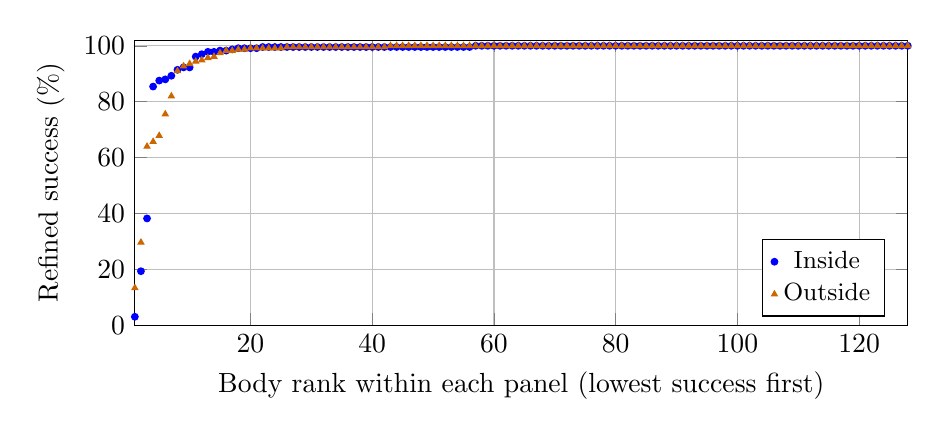
\begin{tikzpicture}
\begin{axis}[width=0.94\linewidth,height=5.2cm,
xlabel={Body rank within each panel (lowest success first)},
ylabel={Refined success (\%)},xmin=1,xmax=128,ymin=0,ymax=102,
legend pos=south east,legend style={font=\small},grid=major]

\addplot[only marks,mark=*,mark size=1.2pt,blue] coordinates {
(1,3.00) (2,19.31) (3,38.20) (4,85.41) (5,87.55) (6,87.98) (7,89.27) (8,91.42) (9,92.27) (10,92.27) (11,96.14) (12,97.00) (13,97.85) (14,97.85) (15,98.28) (16,98.28) (17,98.71) (18,99.14) (19,99.14) (20,99.14) (21,99.14) (22,99.57) (23,99.57) (24,99.57) (25,99.57) (26,99.57) (27,99.57) (28,99.57) (29,99.57) (30,99.57) (31,99.57) (32,99.57) (33,99.57) (34,99.57) (35,99.57) (36,99.57) (37,99.57) (38,99.57) (39,99.57) (40,99.57) (41,99.57) (42,99.57) (43,99.57) (44,99.57) (45,99.57) (46,99.57) (47,99.57) (48,99.57) (49,99.57) (50,99.57) (51,99.57) (52,99.57) (53,99.57) (54,99.57) (55,99.57) (56,99.57) (57,100.00) (58,100.00) (59,100.00) (60,100.00) (61,100.00) (62,100.00) (63,100.00) (64,100.00) (65,100.00) (66,100.00) (67,100.00) (68,100.00) (69,100.00) (70,100.00) (71,100.00) (72,100.00) (73,100.00) (74,100.00) (75,100.00) (76,100.00) (77,100.00) (78,100.00) (79,100.00) (80,100.00) (81,100.00) (82,100.00) (83,100.00) (84,100.00) (85,100.00) (86,100.00) (87,100.00) (88,100.00) (89,100.00) (90,100.00) (91,100.00) (92,100.00) (93,100.00) (94,100.00) (95,100.00) (96,100.00) (97,100.00) (98,100.00) (99,100.00) (100,100.00) (101,100.00) (102,100.00) (103,100.00) (104,100.00) (105,100.00) (106,100.00) (107,100.00) (108,100.00) (109,100.00) (110,100.00) (111,100.00) (112,100.00) (113,100.00) (114,100.00) (115,100.00) (116,100.00) (117,100.00) (118,100.00) (119,100.00) (120,100.00) (121,100.00) (122,100.00) (123,100.00) (124,100.00) (125,100.00) (126,100.00) (127,100.00) (128,100.00)
};\addlegendentry{Inside}
\addplot[only marks,mark=triangle*,mark size=1.2pt,orange!80!black] coordinates {
(1,13.30) (2,29.61) (3,63.95) (4,65.67) (5,67.81) (6,75.54) (7,81.97) (8,90.99) (9,92.70) (10,93.56) (11,94.42) (12,94.85) (13,95.71) (14,96.14) (15,97.42) (16,98.28) (17,98.28) (18,98.71) (19,98.71) (20,99.14) (21,99.14) (22,99.14) (23,99.14) (24,99.14) (25,99.14) (26,99.57) (27,99.57) (28,99.57) (29,99.57) (30,99.57) (31,99.57) (32,99.57) (33,99.57) (34,99.57) (35,99.57) (36,99.57) (37,99.57) (38,99.57) (39,99.57) (40,99.57) (41,99.57) (42,99.57) (43,100.00) (44,100.00) (45,100.00) (46,100.00) (47,100.00) (48,100.00) (49,100.00) (50,100.00) (51,100.00) (52,100.00) (53,100.00) (54,100.00) (55,100.00) (56,100.00) (57,100.00) (58,100.00) (59,100.00) (60,100.00) (61,100.00) (62,100.00) (63,100.00) (64,100.00) (65,100.00) (66,100.00) (67,100.00) (68,100.00) (69,100.00) (70,100.00) (71,100.00) (72,100.00) (73,100.00) (74,100.00) (75,100.00) (76,100.00) (77,100.00) (78,100.00) (79,100.00) (80,100.00) (81,100.00) (82,100.00) (83,100.00) (84,100.00) (85,100.00) (86,100.00) (87,100.00) (88,100.00) (89,100.00) (90,100.00) (91,100.00) (92,100.00) (93,100.00) (94,100.00) (95,100.00) (96,100.00) (97,100.00) (98,100.00) (99,100.00) (100,100.00) (101,100.00) (102,100.00) (103,100.00) (104,100.00) (105,100.00) (106,100.00) (107,100.00) (108,100.00) (109,100.00) (110,100.00) (111,100.00) (112,100.00) (113,100.00) (114,100.00) (115,100.00) (116,100.00) (117,100.00) (118,100.00) (119,100.00) (120,100.00) (121,100.00) (122,100.00) (123,100.00) (124,100.00) (125,100.00) (126,100.00) (127,100.00) (128,100.00)
};\addlegendentry{Outside}
\end{axis}\end{tikzpicture}
\caption{All 128 bodies in each unseen panel, independently sorted by
original-checkpoint success on the same 233 known clips. Ranking is
panel-specific and does not pair inside and outside bodies. Severe failures
are retained alongside the near-ceiling majority.}\label{fig:unseen_v2_shapes}
\end{figure}


\subsubsection{Coefficient tiers and physical-property groups}
\begin{table}[t]
\centering\small
\caption{Predefined outside coefficient tiers and descriptive simulated-mass
bins on the 233-clip panel. Tier and mass rows overlap; each partition covers
all 128 bodies. Mass thresholds are the trained-asset range. These are
associations, not identified causes.}\label{tab:unseen_v2_groups}
\begin{tabular}{lrrr}
\toprule
Group & Bodies & Refined (\%) & Full-data (\%) \\
\midrule
$\|\beta\|_\infty\in(3,3.5]$ & 32 & 99.03 & 99.46 \\
$\|\beta\|_\infty\in(3.5,4]$ & 32 & 97.76 & 97.81 \\
$\|\beta\|_\infty\in(4,4.5]$ & 32 & 95.33 & 95.12 \\
$\|\beta\|_\infty\in(4.5,5]$ & 32 & 96.47 & 97.87 \\
\midrule
Mass $<26.4$ kg & 2 & 100.00 & 100.00 \\
Mass $26.4$--$144.4$ kg & 118 & 98.33 & 98.13 \\
Mass $>144.4$ kg & 8 & 79.02 & 88.62 \\
\bottomrule
\end{tabular}
\end{table}
Success does not decline monotonically across coefficient tiers
(Table~\ref{tab:unseen_v2_groups}). The eight heaviest outside bodies have
lower mean success, but small, overlapping property groups and paired
male/female templates are not independent samples of physical-property
space. Bodies outside the trained height range perform well on average
(97.91\% outside; 96.42\% inside), while the tallest in-range bin is weaker
(90.53\% outside; 88.75\% inside). Raw coefficient extremity, mass, and
height therefore do not provide a simple ordering of transfer difficulty.

\subsubsection{Checkpoint sensitivity: gains and regressions}
Full-data changes exceed the identical-checkpoint rerun magnitude and have
clip-bootstrap intervals excluding zero in all three headline populations.
This supports a measurable change between these two checkpoints, not a
causal claim about training duration or coverage, which changed together.
Ordinary checkpoint variation remains unmeasured.

Outside improvement is concentrated in the ten bodies outside the trained
mass range ($+7.68$ pp, 95\% CI [$+6.39$, $+9.01$]) and the highest
coefficient tier ($+1.39$ pp [$+1.07$, $+1.72$]). Yet outside mean position
error increases by 2.4\,mm overall; inside and control increases are 5.0 and
3.1\,mm. Threshold success and continuous tracking quality move differently.
The gain therefore does not establish uniformly tighter tracking.

\begin{table}[t]
\centering\small
\caption{All bodies whose paired success-change interval lies entirely below
$-2$ percentage points on the 233-clip panel. These exploratory per-body
intervals are not adjusted for multiple comparisons.}\label{tab:unseen_v2_regressions}
\begin{tabular}{llrrr}
\toprule
Panel & Asset & Refined (\%) & Full-data (\%) & $\Delta$ (pp) \\
\midrule
Inside & \texttt{female\_e7bc8c92} & 92.3 & 79.0 & $-13.30$ \\
Inside & \texttt{male\_6d81a8f6} & 97.9 & 85.0 & $-12.88$ \\
Inside & \texttt{male\_ec3bb7f8} & 19.3 & 10.7 & $-8.58$ \\
Outside & \texttt{female\_edcf2449} & 94.8 & 58.4 & $-36.48$ \\
Outside & \texttt{male\_a7f6b877} & 65.7 & 40.8 & $-24.89$ \\
Outside & \texttt{male\_edcf2449} & 82.0 & 67.0 & $-15.02$ \\
Outside & \texttt{female\_e706da88} & 94.4 & 79.8 & $-14.59$ \\
Outside & \texttt{female\_bd0ec1ce} & 63.9 & 52.8 & $-11.16$ \\
Outside & \texttt{female\_f9bf3075} & 97.4 & 88.8 & $-8.58$ \\
\bottomrule
\end{tabular}
\end{table}
Three inside and six outside bodies meet the regression rule
(Table~\ref{tab:unseen_v2_regressions}); no trained control body does.
Five outside bodies have intervals entirely above $+2$ pp, including
\texttt{female\_98d4329d} (29.6\% to 94.8\%) and
\texttt{male\_1c099619} (13.3\% to 71.2\%). The weakest inside body improves
only to 8.6\%. Neither improved extremes nor a higher outside average
justify calling full-data a uniformly better controller.

The separate 23-clip validation/test subset gives inside success
97.08\% versus 96.50\%, and outside 96.81\% versus 96.91\% for refined and
full-data. Full-data trained on these identities; these values are diagnostic,
not untouched motion generalisation, and are excluded from the headline.

\pending{Audit per-asset reference feasibility and inspect first-threshold
crossings on severe failures and successful counterparts. Add contact,
root-height, and actuation traces before distinguishing reference,
controller, or asset mechanisms.}

\subsection{RQ3: Design support and trade-offs}
\subsubsection{Architecture trade-offs across training seeds}\label{sec:architecture_results}
Each refined-reference architecture has three seeds. Each run contributes
one last-eight-evaluation summary (epochs 4,600--6,000); uncertainty below is
sample standard deviation across three summaries. Seed-1/2 values were checked
against local TensorBoard records. Seed-0 values are retained from the
historical table; their original logs were not independently available in that check.

\begin{table}[t]
\centering\small
\caption{Three-seed refined-reference development comparison. Success and
jerk are mean $\pm$ sample standard deviation across seeds; position and
rotation are across-seed means.}\label{tab:architecture_seeds}
\begin{tabularx}{\linewidth}{@{}Yrrrr@{}}
\toprule
Architecture & Success (\%) & Pos. (m) & Rot. (rad) & Jerk \\
\midrule
A: temporal MLP & $95.14\pm2.07$ & 0.118 & 0.216 & $2{,}110\pm643$ \\
B: temporal attention & $97.56\pm0.34$ & 0.090 & 0.218 & $2{,}783\pm887$ \\
C: slot/type attention & $97.89\pm0.22$ & 0.090 & 0.219 & $2{,}413\pm762$ \\
D: C + adaLN-Zero & $97.17\pm0.08$ & 0.083 & 0.211 & $2{,}659\pm674$ \\
\bottomrule
\end{tabularx}
\end{table}

C has the highest mean success; D has the lowest position and rotation errors;
A has the lowest mean jerk. No model dominates. Jerk ordering changes across
seeds, so the apparent factor-of-two advantage in seed 0 is not a consistent
architecture effect. Three seeds do not establish statistical superiority
from small success differences. We retain C as a practical compromise.
These reruns support the already-trained full-scale model rather than
establishing selection before training. Capacities and runtimes differ
(Appendix~\ref{app:history}).

\subsubsection{Reference refinement: artifact reduction and fidelity}\label{sec:refinement_results}

A paired reference audit supports reduced sliding and penetration with
small pose/root changes, at the cost of higher reference jerk. Policy
comparisons do not establish a causal benefit or absence of quality cost.

The reference-level part is an offline before/after audit on the packaged
motion tensors, with no simulation, over all 19,200 references of the 150-clip
development set (150 clips $\times$ 128 body configurations).
Table~\ref{tab:refine_audit} reports the artifact measures -- stance-foot
horizontal speed during detected contact, the fraction of frames whose lowest
body centre is below the floor, and reference-domain position jerk -- and the
fidelity measures -- per-body geodesic rotation change, root horizontal
displacement, and the cross-shape variance of per-shape knee-flexion range,
which must be preserved rather than flattened.

\begin{table}[t]
\centering
\small
\caption{Reference-refinement audit over all 19,200 development references.
Artifact rows: corpus mean before and after, and the fraction of individual
motions that improve; the per-motion distributions are in
Figure~\ref{fig:refine_dist}. Fidelity rows: corpus mean of the
refined-vs-unrefined difference. Jerk is the raw mean third-difference of body
positions, not the windowed evaluator score.}\label{tab:refine_audit}
\begin{tabularx}{\linewidth}{@{}Yrrr@{}}
\toprule
& Unref.\ mean & Refined mean & Motions improved \\
\midrule
Stance-foot speed (m/s) $\downarrow$ & 0.055 & 0.038 & 96\% \\
Frames below floor (\%) $\downarrow$ & 39.6 & 3.3 & 45\% \\
Frames within 2\,cm of floor (\%) $\downarrow$ & 49.8 & 33.6 & --- \\
Position jerk (m/s$^3$) & 45.2 & 60.7 & 21\% \\
\midrule
Per-body rotation change (deg) & \multicolumn{3}{c}{0.12} \\
Root horizontal displacement (m) & \multicolumn{3}{c}{0.008} \\
Cross-shape var., knee-flexion range (ratio r/u) & \multicolumn{3}{c}{0.94} \\
\bottomrule
\end{tabularx}
\end{table}

\begin{figure}[t]
\centering
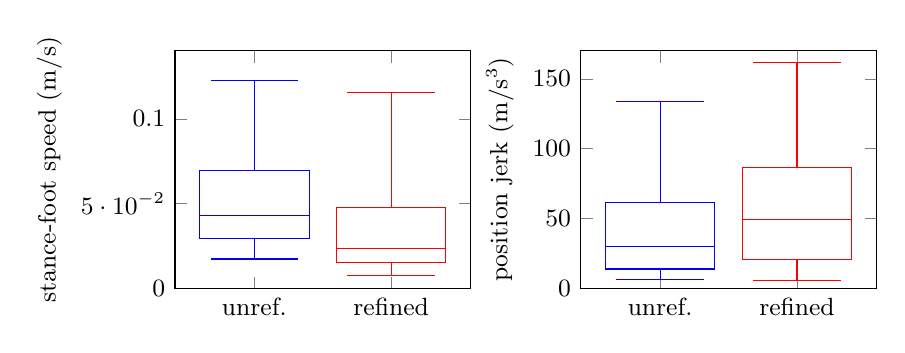
\begin{tikzpicture}
\begin{groupplot}[
  group style={group size=2 by 1, horizontal sep=1.4cm},
  width=0.44\linewidth, height=4.6cm,
  boxplot/draw direction=y, xtick={1,2}, xticklabels={unref., refined},
  tick label style={font=\small}, label style={font=\small},
]
\nextgroupplot[ylabel={stance-foot speed (m/s)}, ymin=0, ymax=0.14]
\addplot+[boxplot prepared={lower whisker=0.0174, lower quartile=0.0294,
  median=0.0430, upper quartile=0.0695, upper whisker=0.1228}] coordinates {};
\addplot+[boxplot prepared={lower whisker=0.0078, lower quartile=0.0151,
  median=0.0237, upper quartile=0.0476, upper whisker=0.1157}] coordinates {};
\nextgroupplot[ylabel={position jerk (m/s$^3$)}, ymin=0, ymax=170]
\addplot+[boxplot prepared={lower whisker=6.5, lower quartile=14.0,
  median=30.4, upper quartile=61.6, upper whisker=133.5}] coordinates {};
\addplot+[boxplot prepared={lower whisker=5.7, lower quartile=20.8,
  median=49.2, upper quartile=86.7, upper whisker=161.6}] coordinates {};
\end{groupplot}
\end{tikzpicture}
\caption{Per-motion distributions (box: quartiles; whiskers: 5th--95th
percentile) over the 19,200 development references. Foot-skate drops across
almost the whole distribution; position jerk rises across almost the whole
distribution.}\label{fig:refine_dist}
\end{figure}

Refinement lowers stance-foot speed from 0.055 to 0.038\,m/s, with 96\%
of references improving, and below-floor frames from 39.6\% to 3.3\%.
Small rotation/root changes and a knee-range variance ratio of 0.94 support
preservation of the measured motion features, not equivalence of all
kinematics. Only 45\% of references improve the below-floor measure because
many were already grounded. The cost is higher reference jerk (45.2 to
60.7\,m/s$^3$); 79\% of references worsen on that measure.
Figure~\ref{fig:refine_dist} shows that both the sliding reduction and jerk
increase extend across the distribution. Temporal root/clearance corrections
are a candidate explanation for the jerk cost, but its contribution to
policy smoothness is not isolated.

The refined/unrefined pairs in Table~\ref{tab:ablation_results} track their
own targets and have one seed per unrefined case. They describe different
tasks. The reference audit justifies cleaning; a stronger policy-level claim
requires a common-reference checkpoint comparison.


\subsubsection{Explicit morphology conditioning: a missing causal control}
Every architecture above receives morphology inputs in both actor and critic.
The adaLN-Zero variant changes their use in the actor; it does not test their
removal. Successful transfer therefore establishes a capability of the whole
system, not that explicit coefficients cause it. Body-dependent state and
reference targets also expose morphology.
\pending{Train a matched controller without explicit morphology inputs using
the same references, body panel, budget, and seeds. Evaluate both policies on
fixed trained- and unseen-body panels. Inference-time masking or shuffling
can supplement this test but introduces distribution shift and cannot replace
it. A common-reference policy comparison is also needed to isolate the
learning effect of refinement.}

\section{Discussion and Limitations}\label{sec:discussion}
The three questions distinguish a capability from its coverage and mechanism.
RQ1 establishes shared tracking of held-out motions on selected trained
bodies and execution across all trained bodies on development clips. RQ2
establishes high average transfer on both sides of the training coefficient
boundary, while exposing bodies for which tracking largely fails. RQ3
supports practical architecture and reference-processing choices, but not a
causal explanation of transfer.

\paragraph{Average transfer and individual robustness.}
Similar inside/outside averages do not make body extrapolation uniformly
reliable. Tier success is non-monotonic, and poor tracking occurs both beyond
and within the training mass/height ranges. These simulated properties
describe the tested assets; their associations do not identify failure causes.
The later checkpoint recovers some bodies and substantially harms others.
Its outside success gain accompanies a slight increase in mean position
error, so threshold success alone would overstate the improvement.

\paragraph{Coverage and inference.}
The unseen-body headline uses known motion identities to isolate body
transfer. The separate 23 validation/test clips cannot provide an untouched
motion test for the full-data checkpoint, which trained on them. The
1,048-clip independent test uses one trained body per clip; a fixed
held-out-motion panel crossed with all 128 trained bodies remains missing.
Original/mirrored variants stay together, but the splits are not demonstrated
to be subject- or recording-disjoint. Clip-bootstrap intervals hold the body
panel fixed and do not quantify uncertainty over shape space. One full-scale
training run and one candidate checkpoint do not measure training-seed or
ordinary checkpoint variation. Identical-checkpoint reruns measure simulator
variability, with nearly cancelling pooled changes but appreciable pair flips.

\paragraph{Mechanism and design.}
State and reference observations already carry shape information. A matched
policy without explicit morphology inputs is needed to attribute transfer to
those inputs. The architecture comparison keeps them in every model and has
unequal capacities. Refinement reduces contact artifacts with small pose
changes but raises target jerk; policies evaluated against different targets
do not isolate its learning benefit. The exploratory physical analysis in
Appendix~\ref{sec:physics} remains descriptive pending a clip-level contrast.

\paragraph{Failure diagnosis and scope.}
The unseen-body runs detect error-threshold failures, and all failed rows have zero termination flags. Those flags alone do not
prove absence of falls; their interpretation depends on the replay
configuration. Synchronized rollouts, contact/root trajectories, and reference-quality
audits are needed before assigning a failure mechanism. Extreme HUMOS
references have been refined but lack per-asset feasibility validation.
Estimated masses, collision proxies, and mass-scaled gains are modeling
choices; tracking success and jerk do not certify biomechanical realism.
The short, reference-initialized flat-ground protocol excludes objects,
partners, long-horizon recovery, skeletal-topology changes, and real robots.

The corpus is derived: clip/body variants are not independent captures.
Caption alignment, immutable generation checksums, and redistribution
permissions require auditing before a benchmark-release claim. A matched
external tracker would strengthen comparative conclusions, but the published
capability table alone cannot establish a performance advantage.

\section{Conclusion}\label{sec:conclusion}
We study shared physics-based imitation through paired morphology-specific
references and assets, a temporal controller, and explicit separation of
motion and body exposure. For RQ1, one policy trained across 128 bodies
achieves 99.14\% success on held-out motions with one selected trained body
per clip. For RQ2, it achieves 97.28\% inside-range and 97.15\% outside-range
unseen-body success, but individual bodies can fail on most clips and a later
checkpoint introduces both recoveries and regressions. For RQ3, repeated
architecture comparisons and paired reference audits identify tracking,
smoothness, and contact-quality trade-offs rather than a dominant design.
The evidence supports strong average shared tracking and transfer within
this protocol. All-body held-out-motion coverage, matched conditioning and
external controls, and dynamic diagnosis of severe failures remain necessary
for stronger claims about robustness and mechanism.


\appendix
\section{Reproducibility Details}\label{app:reproducibility}

\subsection{Source preparation and refinement settings}\label{app:preprocessing}

The AMASS source collections used by the preparation pipeline are ACCAD,
BioMotionLab\_NTroje, BMLhandball, BMLmovi, CMU, DFaust\_67, EKUT,
Eyes\_Japan\_Dataset, HumanEva, KIT, MPI\_HDM05, MPI\_Limits, MPI\_mosh,
SFU, SSM\_synced, TCD\_handMocap, TotalCapture, and Transitions\_mocap.
Source preparation operates at 20\,Hz; the final motion libraries use
30\,Hz. Joint ordering and quaternion conventions must follow the matching
asset and MotionLib conversion rather than be inferred from source array
positions.

\begin{table}[htbp]
\centering
\small
\caption{Default settings of the current reference-refinement procedure.
Frame counts refer to the 30\,Hz MotionLib representation. These are
kinematic-processing settings, not physical constraints learned by the policy.}\label{tab:refinement_parameters}
\begin{tabularx}{\linewidth}{@{}lY@{}}
\toprule
Operation & Setting \\
\midrule
Contact candidates & Left/right ankle and toe bodies \\
Contact detection thresholds & Speed 0.15\,m/s; height 0.10\,m \\
Contact cleanup & Close gaps up to 2 frames; remove runs shorter than 3 frames \\
Rotation filter & Savitzky--Golay, 9-frame window, polynomial order 3 \\
Rotation blend / bound & Strength 0.5; maximum geodesic correction $8^\circ$ \\
Contact-transition guard & Separate segments; 2-frame transition taper \\
Root XY correction & Median stance anchors; least-squares common translation \\
Root correction regularization & 21-frame smoothing window; 0.10\,m displacement cap \\
Ground clearance & 0.005\,m collision-geometry margin; 5-frame lift smoothing \\
Final reconstruction & Per-asset FK and per-motion velocity recomputation \\
\bottomrule
\end{tabularx}
\end{table}

\subsection{PD gains and limits}\label{app:control}

Table~\ref{tab:pd_parameters} gives the base values configured for the
SMPL morphology robot. For joint $d$ belonging to rigid body $j$, the
simulator applies the multiplier
\begin{equation}
    \rho_{b,j} = \frac{m_{b,j}}{m_{\mathrm{ref},j}}
\end{equation}
to stiffness, damping, and effort limit. The velocity limit is not mass-scaled.
All relevant asset masses, joint ranges, collision settings, and the reference
asset must accompany a reproducible physical interpretation.

\begin{table}[htbp]
\centering
\small
\caption{Base PD and actuation values before per-body mass scaling.
Stiffness and damping use the simulator's rotational PD units
(Nm/rad and Nm\,s/rad); effort limits are in Nm and velocity limits in rad/s.}\label{tab:pd_parameters}
\begin{tabular}{lrrrr}
\toprule
Joint family & Stiffness & Damping & Effort limit & Velocity limit \\
\midrule
Hip, knee, ankle & 800 & 80 & 500 & 100 \\
Toe & 500 & 50 & 500 & 100 \\
Torso, spine, chest & 1,000 & 100 & 500 & 100 \\
Neck, head, thorax, shoulder, elbow & 500 & 50 & 500 & 100 \\
Wrist, hand & 300 & 30 & 500 & 100 \\
\bottomrule
\end{tabular}
\end{table}

\subsection{Windowed jerk convention}\label{app:smoothness}

The logged smoothness score is computed from simulated global body positions
using consecutive finite differences with control interval
$\Delta t=1/30$\,s. A nominal 0.4\,s window contains
$W=\max(4,\lfloor0.4/\Delta t\rfloor)$ frames, giving $W=12$ at the
configured rate and duration $T_w=(W-1)\Delta t$. For body $j$ in window $w$,
let $L_{w,j}$ be the sum of speed times $\Delta t$ and let
$\dddot{p}_{w,j}$ denote the third finite difference. The implementation uses
\begin{equation}
    J_{w,j} =
    \frac{T_w^5
      \sum_{t\in w}\|\dddot{p}_{t,j}\|_2^2\,\Delta t}
    {\max(L_{w,j},\epsilon)^2+\epsilon},
    \qquad \epsilon=0.1,
    \label{eq:jerk}
\end{equation}
where the sum includes the valid third-difference samples in the window.
Window scores are averaged per body and then across bodies and motions.
High-jerk percentage counts windows for which
$\max_j J_{w,j}>6{,}500$.

Equation~\eqref{eq:jerk} documents the existing numerical convention, including
its regularizers; it is not presented as a universally dimensionless or
sampling-rate-invariant biomechanical measure. Comparisons must keep the
sample rate, window, units, regularizers, and aggregation fixed. Reference
refinement reports also include raw jerk in m/s$^3$; those values are a
different metric and cannot be compared numerically to this logged score.

\subsection{Split and experiment provenance}\label{app:provenance}

The split metadata is stored in
\path{data/splits/hhi_stage2_v1/split_metadata.json}, with schema version 1,
split seed 42, and split identifier
\begin{quote}
\footnotesize\ttfamily
4c1c9d592e3dbeef15abe18cb50a3141820735849414ecc2d8959e9f38502263
\end{quote}
It records the source-manifest hash, training/validation/test manifest and
ID-list hashes, difficulty information, and the forced training reservation.
The generator uses 100 difficulty strata; the 150 requested development
identities expand to 286 retained identities when existing mirrored partners
are included. Checkpoint/run split provenance refers to these artifacts,
not just a verbal 90/5/5 ratio.

The documented HUMOS configuration selects
\path{logs/humos/q6zbv2tu/checkpoints/latest-epoch=1599.ckpt}. The immutable
HUMOS checkpoint checksum and the SMPLSim / asset-generation revision hashes
are to be archived with the dataset release; a checkpoint path identifies the
local workflow but is not a substitute for a checksum.

The principal implementation entry points are:
\begin{itemize}
    \item Reference refinement:
    \path{tools/refine_humos_motion.py}; streamed per-clip processing:
    \path{tools/refine_humos_r2_per_clip.py}.
    \item Selected full-scale experiment:
    \path{examples/experiments/mimic/mlp_wide_stage2_discover_attention_slot_type.py},
    inheriting the common attention experiment and enabling slot/type embeddings.
    \item Corrected development comparison:
    \path{tools/train_150_evalfix_ablation.sh} (cases A--E) and
    \path{tools/train_150_evalfix_unrefined.sh} (cases F--H), seed 0.
    \item Motion residency and evaluation:
    \path{protomotions/components/global_clip_pool.py} and
    \path{protomotions/agents/evaluators/mimic_evaluator.py}.
    \item Standalone split evaluation:
    \path{evaluate_validation_split.py} and \path{evaluate_test_split.py}
    under \path{protomotions/}. Each output records the checkpoint, split,
    reference version, and shape panel; the test evaluator additionally
    checks the test-manifest hash, count, and disjointness before running.
\end{itemize}

\subsection{Unseen-body and repeated-seed evidence}
The sole unseen-body study is the inside/outside replay of 9 October 2026.
Its source report is \path{r2:proto-data/unseen_shapes_v2/eval/REPORT.md};
a local read-only snapshot is retained under
\path{paper-draft/evidence/unseen_shapes_v2/}, including both 128-row
per-shape CSVs, comparison summaries, checkpoint identities, and rerun checks.
The evaluator is \path{tools/analyze_unseen_morphology_generalization.py};
paired analysis uses \path{tools/compare_checkpoints_unseen_morphology.py}.
The report records code revision \texttt{75324d9} at analysis time.

Frozen checkpoint SHA-256 values are:
\begin{quote}\footnotesize\ttfamily
refined (epoch 28,170):\\
\detokenize{4b83f20c93bf95fab389fc8935685ef8a2c7e46583f765e8c802421edb4479cb}\\
fulldata (epoch 34,000):\\
\detokenize{7b57de8ec047c390c2881f8a630d7196a09da6dd08bfbae743f36d6542cd2192}
\end{quote}
Each checkpoint has its own frozen resolved inference configuration.
All per-pair outputs and logs remain on R2; the local small-artifact snapshot
is not a copy of the complete rollout records. The 233/23 clip partition,
body manifests, and physical-property groups are defined in the source report.

Seed-1/2 architecture records are in the corresponding
\path{results/hhi_150_evalfix_A_seed1} through
\path{results/hhi_150_evalfix_D_seed2} run folders. Resumed logging segments
must be joined by evaluation epoch before forming last-eight summaries.
Across-seed standard deviation is computed from three run summaries, rather
than from all scheduled evaluations pooled as independent observations.

For each final experiment, retain the resolved configuration, code revision,
model/checkpoint checksum, body coefficient and asset manifests, split hashes,
all resume segments, frame count, GPU model/count, and elapsed GPU-hours.
For each evaluation, retain per-pair clip and asset IDs, panel selection,
success/failure, valid horizon, and component errors in a local analysis file.
The main full-scale W\&B identifier is \texttt{3mvgad6f}; the corrected
small-scale group is \texttt{hhi\_150\_evalfix\_comparison}.
The evaluation/sampling correction is recorded in commit \texttt{3685247}.

\pending{Two items remain before a finalized benchmark report: the immutable
HUMOS/SMPLSim checksums (to be archived with the dataset release) and the
release of the retained per-motion evaluation records for the validation and
test splits.}

\section{Development and Training Provenance}\label{app:history}
RQ1 uses the original epoch-28,170 checkpoint; RQ2 also compares the frozen
epoch-34,000 candidate. The monitoring
snapshot below is a separate measurement at epoch 28,159. Historical
single-seed comparisons and compute records are retained here to distinguish
provenance from final performance.
\subsection{Recorded full-scale validation result}\label{sec:full_results}

Table~\ref{tab:full_results} reports the final scheduled monitoring evaluation
recorded for the selected full-scale slot/type run, at epoch 28,159 after
approximately 11.07 billion simulated frames. The separately downloaded
checkpoint is from epoch 28,170. These values are post-correction,
morphology-matched evaluations, not measurements of that later checkpoint
or of the independent test split.

\begin{table}[t]
\centering
\small
\caption{Recorded full-scale monitoring snapshot. Validation contains
1,048 held-out clips; each evaluation uses one selected trained body per clip.
The active resident pool is difficulty-biased. Values are the stored
distributed logging summaries from run \texttt{3mvgad6f}, epoch 28,159;
no confidence intervals or all-shape coverage are implied.}\label{tab:full_results}
\begin{tabular}{lrr}
\toprule
Metric & Hard resident pool & Validation holdout \\
\midrule
Success rate (\%) $\uparrow$ & 89.84 & 98.47 \\
Mean body-position error (m) $\downarrow$ & 0.0960 & 0.0698 \\
Mean global body-rotation error (rad) $\downarrow$ & 0.2261 & 0.1760 \\
Mean maximum-joint position error (m) $\downarrow$ & 0.1848 & 0.1412 \\
Windowed normalized jerk $\downarrow$ & 1,442.8 & 1,151.7 \\
High-jerk windows (\%) $\downarrow$ & 31.05 & 27.25 \\
\bottomrule
\end{tabular}
\end{table}

The validation score is higher than the resident-pool score, while the
reported errors are lower. This comparison is consistent with a curriculum
that concentrates residency on difficult clips: the resident pool is not an
independent uniform sample of the training distribution. Its 89.84\% success
rate should not be interpreted as the success rate of the entire training
corpus, nor should the difference be described as validation outperforming
an IID training sample.

\begin{figure}[t]
\centering
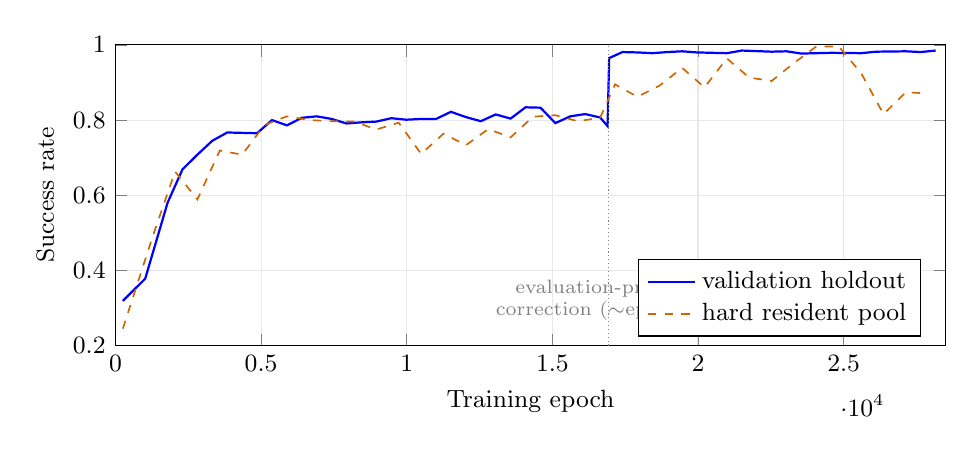
\begin{tikzpicture}
\begin{axis}[
  width=\linewidth, height=5.4cm,
  xlabel={Training epoch}, ylabel={Success rate},
  xmin=0, xmax=28500, ymin=0.2, ymax=1.0,
  legend pos=south east, legend cell align=left, legend style={font=\small},
  tick label style={font=\small}, label style={font=\small},
  grid=both, grid style={gray!18},
]
\addplot[thick, blue] coordinates {
(255,0.319)(1023,0.378)(1791,0.580)(2303,0.669)(2815,0.708)(3327,0.745)
(3839,0.767)(4351,0.766)(4863,0.765)(5375,0.800)(5887,0.786)(6399,0.806)
(6911,0.810)(7423,0.803)(7935,0.791)(8447,0.794)(8959,0.796)(9471,0.805)
(9983,0.801)(10495,0.803)(11007,0.803)(11519,0.822)(12031,0.808)(12543,0.797)
(13055,0.815)(13567,0.804)(14079,0.834)(14591,0.833)(15103,0.792)(15615,0.810)
(16127,0.816)(16639,0.807)(16895,0.784)(16950,0.965)(17407,0.981)(17919,0.980)
(18431,0.978)(18943,0.981)(19455,0.983)(19967,0.980)(20991,0.978)(21503,0.985)
(22527,0.982)(23039,0.983)(23551,0.977)(24575,0.979)(25599,0.978)(26111,0.982)
(27135,0.983)(27647,0.981)(28159,0.985)
};
\addlegendentry{validation holdout}
\addplot[semithick, orange!80!black, dashed] coordinates {
(255,0.245)(1279,0.490)(2047,0.663)(2815,0.589)(3583,0.719)(4351,0.708)
(5119,0.787)(5887,0.810)(6655,0.800)(7423,0.797)(8191,0.796)(8959,0.775)
(9727,0.793)(10495,0.710)(11263,0.764)(12031,0.733)(12799,0.776)(13567,0.754)
(14335,0.809)(15103,0.813)(15871,0.797)(16639,0.806)(17151,0.895)(17919,0.862)
(18687,0.892)(19455,0.939)(20223,0.887)(20991,0.964)(21759,0.913)(22527,0.904)
(23295,0.952)(24063,0.996)(24831,0.996)(25599,0.925)(26367,0.816)(27135,0.874)
(27903,0.871)
};
\addlegendentry{hard resident pool}
\draw[gray, densely dotted] (axis cs:16920,0.2) -- (axis cs:16920,1.0);
\node[anchor=south, font=\scriptsize, gray, align=center]
  at (axis cs:16920,0.24) {evaluation-protocol\\correction ($\sim$ep.\ 16.9k)};
\end{axis}
\end{tikzpicture}
\caption{Scheduled success rate over training for the full-scale slot/type
run (\texttt{3mvgad6f}). The step near epoch 16.9k is the morphology-matched
evaluation correction plus its sampling change, not an instantaneous learning
event; pre-correction points use the earlier, sometimes mismatched
reference-to-asset assignment and are not comparable to the post-correction
curve. After the correction the holdout success rate climbs from about
0.96 to a stable 0.98--0.985. The resident-pool curve is noisier because
residency is continually re-concentrated on hard clips.}\label{fig:learning_curve}
\end{figure}

The 98.47\% result supports strong tracking of the selected held-out
clip/body pairs under the specified threshold. It does not establish
all-body success for those clips, unseen-body generalization, or an untouched
test-set score. The thresholded success rate is complemented by position,
rotation, and smoothness measures because a successful rollout can still
have visible local errors or jitter.

% Evidence: note/README.note.md, section 76, recorded 2026-09-07.
% Do not replace the monitoring epoch with last.ckpt's epoch.
The run record is available at
\href{https://wandb.ai/yugoamaryl/hhi-protomotions/runs/3mvgad6f}
{the full-scale W\&B run}. The current table uses the recorded snapshot,
not a newly executed evaluation.


\subsection{Historical single-seed reference grid}
Cases A--D use refined references and E--H use unrefined references.
Within-run variation must not be interpreted as uncertainty across training
runs. The main architecture conclusion uses repeated refined runs instead.
\begin{table}[t]
\centering
\small
\caption{Historical seed-0 development grid. Success uncertainty is variation across eight evaluations within each run. Other columns are their means. Refined and unrefined policies track different targets. The three-seed comparison is in Table~\ref{tab:architecture_seeds}.}\label{tab:ablation_results}
\begin{tabularx}{\linewidth}{@{}llYrrrr@{}}
\toprule
Case & Architecture / data & Success (\%) & gt err & gr err & Jerk & HJ\% \\
\midrule
A & temporal MLP, refined        & 97.5 $\pm$ 0.8 & 0.109 & 0.207 & 1{,}729 & 33.3 \\
B & attention, refined           & 97.5 $\pm$ 1.4 & 0.098 & 0.228 & 3{,}455 & 40.4 \\
C & slot/type, refined           & \textbf{98.1 $\pm$ 0.6} & 0.097 & 0.226 & \textbf{1{,}757} & 34.2 \\
D & slot/type + AdaLN, refined   & 97.1 $\pm$ 1.2 & \textbf{0.090} & 0.220 & 3{,}145 & 38.9 \\
E & slot/type, unrefined         & 97.9 $\pm$ 0.6 & 0.102 & 0.219 & 1{,}422 & 29.6 \\
F & temporal MLP, unrefined      & 96.2 $\pm$ 1.6 & 0.115 & 0.212 & 2{,}927 & 36.6 \\
G & attention, unrefined         & 97.8 $\pm$ 1.2 & 0.098 & 0.219 & 3{,}117 & 34.9 \\
H & slot/type + AdaLN, unrefined & 97.5 $\pm$ 0.9 & 0.091 & 0.207 & 2{,}956 & 34.0 \\
\bottomrule
\end{tabularx}
\end{table}
\subsection{Compute accounting}
We retain W\&B logs, resolved configurations, checkpoint epochs, and local
results for compute accounting. Small-scale development and full-scale
training costs should be reported separately, including resumed segments and
failed launches when discussing practical cost. GPU-hours, rather than
epoch counts alone, quantify this budget.

Table~\ref{tab:compute_accounting} reports parameter counts and single-A40
wall-clock cost for the eight corrected 150-clip runs, all completed at the
6,000-epoch budget. Parameter counts are computed analytically from
each run's resolved model configuration (encoder, transformer or flat-MLP,
and head widths), not read from a stored checkpoint file, since every linear
layer in this codebase is instantiated with \texttt{nn.LazyLinear} and has no
fixed parameter count outside a materialized model. Parameter count is set by
the architecture only, so the refined/unrefined pairs share a count
(A/F, B/G, C/E, D/H).

\begin{table}[t]
\centering
\small
\caption{Parameter counts and single-GPU wall-clock cost for the eight
corrected 150-clip runs (seed 0, one A40 each, 6,000 epochs). Actor and
critic are separate networks with independent parameters.}\label{tab:compute_accounting}
\begin{tabularx}{\linewidth}{@{}llrrrY@{}}
\toprule
Case & Arch & Actor params & Critic params & Total params & GPU-h \\
\midrule
A / F & temporal MLP        & 57,349,557 & 8,524,801 & 65,874,358 & 15.8 / 14.4 \\
B / G & attention           & 45,430,197 & 5,800,705 & 51,230,902 & 23.5 / 21.5 \\
C / E & slot/type           & 45,434,037 & 5,804,545 & 51,238,582 & 23.7 / 23.9 \\
D / H & slot/type + adaLN   & 46,256,053 & 5,804,545 & 52,060,598 & 23.9 / 22.4 \\
\bottomrule
\end{tabularx}
\end{table}

Two consequences run against a naive intuition. First, the temporal MLP has
the most total parameters of any architecture, not the fewest: its actor's
first layer reads the full raw concatenation of every observation category
(5,248 dimensions) directly, which alone costs more parameters than the
attention models' three token encoders and transformer combined. The
attention models compress that same information to a 256-dimensional token
per source before the shared final head, trading parameters for the added
transformer computation. Second, despite having more parameters, the temporal
MLP is the fastest to train by a wide margin (15.8/14.4 vs.\ 21.5--23.9
GPU-hours) -- parameter count does not predict wall-clock cost here, since the
attention models pay for multiple sequential module calls (three encoders,
then a transformer stack) rather than one large matrix multiplication chain.
Actor-only adaLN-Zero adds a small but non-negligible cost over slot/type
(roughly 822,000 actor parameters from the per-layer modulation networks and
morphology encoder), a capacity difference rather than evidence of a smoothness benefit.

The full-scale selected run shares C and E's architecture exactly (same
encoder, transformer, and head widths;
\texttt{mlp\_wide\_stage2\_discover\_attention\_slot\_type.py} inherits
these constants unchanged from the 150-clip experiment file), so its
parameter count is also 51,238,582. It ran on six A40 GPUs
(\texttt{ddp}, 32-bit, 2,048 environments and an 8,192 minibatch per GPU) for
roughly 28,170 epochs. The logged rank-0 wall time is about 77\,h, of which
one interruption near epoch 760 accounts for about 3\,h, giving on the order
of 450 GPU-hours; the run is not directly comparable to the eight matched
single-GPU development runs. An early restart after a memory-related failure
resumed from the last checkpoint with the resident pool reduced from 256 to
128 clips per rank and the local cache multiplier set to 1.0; because
configs are reloaded from the pickle on resume, the frozen configuration
still records the pre-restart pool size of 256. The earlier failed launch was
logged into the same run and is not separately quantifiable.
Segment-level cost accounting remains incomplete. Approximate full-scale
GPU-hours cannot establish superior compute efficiency against the smaller
matched development runs.

\section{Exploratory Physical Analysis}\label{sec:physics}
As a secondary question, we examine whether cross-body variability in
control demand differs between dynamic and quasi-static motions. The original
checkpoint is replayed over 150 development clips and all 128 trained bodies
(19,200 pairs, zero recorded failed episodes). Torque, power, and jerk describe
the configured simulation/controller, not calibrated human biomechanics.

Inherited captions assign classes by keyword matching. Running, jumping,
and kicking form a dynamic group (25 clips); standing and sitting form a
quasi-static group (37 clips). Other clips are outside this pooled comparison.
We subtract each clip's across-body mean before summarizing spread. A
coefficient of variation is sensitive to small baseline demand, so absolute
residuals are more interpretable for this question. This sensitivity alone
does not prove that a relative difference is merely simulation noise.
\begin{table}[t]
\centering
\small
\caption{Cross-shape variability of control demand, dynamic
(running~+~jumping~+~kicking, $n{=}25$ clips) vs.\ quasi-static
(standing~+~sitting, $n{=}37$ clips) motion classes. Each cell is the
standard deviation of the pooled, per-clip-demeaned residual (absolute
units, clip baseline removed) with a 95\% bootstrap CI resampled at the
clip level (10,000 resamples). The final column retains historical pooled-row Levene tests; correlated body rows prevent class-level interpretation of those values.}\label{tab:physical_analysis}
\begin{tabularx}{\linewidth}{@{}Yrrr@{}}
\toprule
Metric & Dynamic std [95\% CI] & Quasi-static std [95\% CI] & Pooled-row $p$ \\
\midrule
Normalized torque (frac.\ effort limit) & $1.93$ [$1.71$, $2.21$] $\times10^{-4}$ & $2.06$ [$1.86$, $2.30$] $\times10^{-4}$ & $0.10$ \\
Mass-normalized power & 0.292 [0.220, 0.370] & 0.259 [0.210, 0.323] & $1.1\times10^{-7}$ \\
Normalized jerk & 350.2 [283.3, 416.9] & 403.2 [303.3, 513.5] & 0.33 \\
\bottomrule
\end{tabularx}
\end{table}

The descriptive spreads differ modestly and their separate confidence
intervals overlap. Bootstrap intervals resample clips, while the recorded
Levene tests pool correlated body rows. Neither pooled-row significance nor
overlap of separate intervals settles the class-level contrast. The present
analysis is descriptive, not a definitive positive or negative interaction result.

\pending{Estimate the dynamic-minus-quasi-static spread contrast using
clip-level resampling or a clip-level permutation test. Report its interval
and effect size, and check units, class membership, and sensitivity to small
classes before drawing an interaction conclusion.}

\section{Complete Unseen-Body Results}\label{app:unseen_tables}
These tables contain every body from the new inside/outside study on the
233 training-split clips. Success percentages and errors are generated from
the retained per-shape CSVs; input fractions have four-decimal precision.
Errors are per-pair time-averaged mean body-position errors including failures.
Bodies share beta keys across male/female templates; rows are not independent
training replicates. Full coefficient distances and physical properties are
retained in the accompanying CSVs.

\subsection{Inside panel}
\begingroup\scriptsize
\setlength{\tabcolsep}{4pt}
\begin{longtable}{lrrrrrrr}
\caption{Inside unseen bodies: mass in kg, height in m, success in \%,
position error in m. R = refined; F = full-data.}\label{tab:all_inside}\\
\toprule
Asset & Tier & Mass & Height & R success & F success & R error & F error \\
\midrule\endfirsthead
\toprule
Asset & Tier & Mass & Height & R success & F success & R error & F error \\
\midrule\endhead
\midrule\multicolumn{8}{r}{Continued on next page}\\\endfoot
\bottomrule\endlastfoot

\texttt{female\_0012b56d} & --- & 54.3 & 1.21 & 99.57 & 99.57 & 0.0844 & 0.0820 \\
\texttt{female\_004f9229} & --- & 67.8 & 1.25 & 100.00 & 100.00 & 0.0711 & 0.0775 \\
\texttt{female\_03b17a5c} & --- & 61.3 & 1.12 & 100.00 & 100.00 & 0.0734 & 0.0790 \\
\texttt{female\_0cdfe35c} & --- & 74.1 & 1.37 & 100.00 & 99.57 & 0.0732 & 0.0696 \\
\texttt{female\_0df54b49} & --- & 36.9 & 1.33 & 87.55 & 84.98 & 0.1513 & 0.2053 \\
\texttt{female\_15ab6d4d} & --- & 73.8 & 1.17 & 100.00 & 100.00 & 0.1093 & 0.1103 \\
\texttt{female\_16407809} & --- & 55.7 & 1.49 & 100.00 & 99.14 & 0.0676 & 0.0702 \\
\texttt{female\_18ba29ff} & --- & 34.4 & 1.35 & 99.57 & 100.00 & 0.0697 & 0.0682 \\
\texttt{female\_1a6e1d07} & --- & 72.5 & 1.20 & 99.57 & 99.57 & 0.0996 & 0.1011 \\
\texttt{female\_1c7a626a} & --- & 47.3 & 1.24 & 85.41 & 89.27 & 0.1510 & 0.1452 \\
\texttt{female\_1e156a55} & --- & 53.1 & 1.22 & 99.57 & 99.14 & 0.0737 & 0.0709 \\
\texttt{female\_1fe45357} & --- & 43.6 & 1.21 & 98.28 & 99.57 & 0.1011 & 0.0896 \\
\texttt{female\_24099a2a} & --- & 51.7 & 1.26 & 100.00 & 100.00 & 0.0620 & 0.0637 \\
\texttt{female\_2ebacdbc} & --- & 79.9 & 1.39 & 100.00 & 100.00 & 0.0676 & 0.0663 \\
\texttt{female\_2ef69857} & --- & 52.1 & 1.31 & 99.57 & 99.57 & 0.0755 & 0.0683 \\
\texttt{female\_2f5af13e} & --- & 44.1 & 1.23 & 100.00 & 100.00 & 0.0597 & 0.0581 \\
\texttt{female\_31c52305} & --- & 30.3 & 1.24 & 100.00 & 100.00 & 0.0743 & 0.0713 \\
\texttt{female\_33c4b70d} & --- & 36.8 & 1.21 & 100.00 & 100.00 & 0.0633 & 0.0672 \\
\texttt{female\_3c31fbf0} & --- & 136.4 & 1.45 & 100.00 & 100.00 & 0.0871 & 0.0881 \\
\texttt{female\_434ee660} & --- & 99.5 & 1.34 & 100.00 & 99.57 & 0.1381 & 0.1339 \\
\texttt{female\_45b559cc} & --- & 32.9 & 1.16 & 100.00 & 100.00 & 0.0750 & 0.0773 \\
\texttt{female\_4ff946fb} & --- & 51.9 & 1.41 & 99.57 & 99.14 & 0.0702 & 0.0770 \\
\texttt{female\_5175aa4d} & --- & 86.0 & 1.23 & 99.57 & 100.00 & 0.0834 & 0.0817 \\
\texttt{female\_56d0764a} & --- & 90.3 & 1.28 & 100.00 & 100.00 & 0.0800 & 0.0855 \\
\texttt{female\_591e5402} & --- & 71.0 & 1.53 & 100.00 & 99.57 & 0.0746 & 0.0680 \\
\texttt{female\_5d08dfec} & --- & 59.5 & 1.36 & 87.98 & 86.27 & 0.1449 & 0.1660 \\
\texttt{female\_5e15544f} & --- & 37.5 & 1.29 & 100.00 & 99.57 & 0.0673 & 0.0687 \\
\texttt{female\_5ff7533b} & --- & 35.8 & 1.24 & 99.57 & 100.00 & 0.0637 & 0.0631 \\
\texttt{female\_5ff8516d} & --- & 88.8 & 1.31 & 100.00 & 100.00 & 0.0769 & 0.0853 \\
\texttt{female\_669a0fb3} & --- & 57.4 & 1.21 & 99.57 & 99.57 & 0.0740 & 0.0770 \\
\texttt{female\_672c8c6d} & --- & 56.6 & 1.34 & 100.00 & 100.00 & 0.0657 & 0.0634 \\
\texttt{female\_6c43e677} & --- & 34.1 & 1.23 & 100.00 & 100.00 & 0.0628 & 0.0643 \\
\texttt{female\_6d81a8f6} & --- & 95.4 & 1.50 & 99.57 & 99.14 & 0.0882 & 0.0936 \\
\texttt{female\_70844ea8} & --- & 64.3 & 1.22 & 100.00 & 99.57 & 0.0785 & 0.0807 \\
\texttt{female\_762ebd03} & --- & 92.7 & 1.39 & 100.00 & 100.00 & 0.0768 & 0.0806 \\
\texttt{female\_790287d8} & --- & 102.9 & 1.32 & 99.57 & 100.00 & 0.0874 & 0.0903 \\
\texttt{female\_826291a7} & --- & 63.2 & 1.10 & 100.00 & 100.00 & 0.0709 & 0.0796 \\
\texttt{female\_8cd58f76} & --- & 30.5 & 1.30 & 100.00 & 99.14 & 0.1017 & 0.1054 \\
\texttt{female\_8e871d31} & --- & 67.8 & 1.47 & 99.14 & 100.00 & 0.0726 & 0.0698 \\
\texttt{female\_98cc6e5a} & --- & 39.7 & 1.28 & 100.00 & 100.00 & 0.0650 & 0.0651 \\
\texttt{female\_99c4b6d5} & --- & 57.5 & 1.23 & 99.57 & 99.57 & 0.0912 & 0.0864 \\
\texttt{female\_9ae68e9d} & --- & 78.8 & 1.28 & 100.00 & 100.00 & 0.0724 & 0.0791 \\
\texttt{female\_9d5ef2c8} & --- & 68.5 & 1.35 & 99.57 & 99.14 & 0.0684 & 0.0639 \\
\texttt{female\_a32ceac3} & --- & 139.3 & 1.45 & 100.00 & 100.00 & 0.0879 & 0.0860 \\
\texttt{female\_bbc77826} & --- & 70.8 & 1.31 & 100.00 & 99.57 & 0.0674 & 0.0734 \\
\texttt{female\_bd1f406b} & --- & 64.2 & 1.45 & 100.00 & 99.57 & 0.0711 & 0.0691 \\
\texttt{female\_cfc560dc} & --- & 68.8 & 1.13 & 89.27 & 98.28 & 0.1559 & 0.1114 \\
\texttt{female\_cfcf0261} & --- & 66.4 & 1.49 & 100.00 & 100.00 & 0.0698 & 0.0698 \\
\texttt{female\_d2e840d7} & --- & 57.2 & 1.27 & 38.20 & 43.35 & 0.5665 & 0.6623 \\
\texttt{female\_d6e4c929} & --- & 96.0 & 1.35 & 100.00 & 100.00 & 0.0826 & 0.0933 \\
\texttt{female\_dba89a6b} & --- & 63.2 & 1.54 & 99.57 & 100.00 & 0.0728 & 0.0675 \\
\texttt{female\_dbdef8ed} & --- & 79.7 & 1.41 & 100.00 & 99.14 & 0.0727 & 0.0824 \\
\texttt{female\_dd2cbc2b} & --- & 77.7 & 1.34 & 99.57 & 99.57 & 0.0740 & 0.0813 \\
\texttt{female\_dfabb96c} & --- & 60.3 & 1.30 & 100.00 & 100.00 & 0.0691 & 0.0709 \\
\texttt{female\_dff75a62} & --- & 104.1 & 1.46 & 99.57 & 99.14 & 0.0887 & 0.0947 \\
\texttt{female\_e0f2d3b0} & --- & 46.6 & 1.40 & 100.00 & 100.00 & 0.0680 & 0.0655 \\
\texttt{female\_e32ea98f} & --- & 27.7 & 1.26 & 100.00 & 100.00 & 0.0622 & 0.0644 \\
\texttt{female\_e7bc8c92} & --- & 79.5 & 1.32 & 92.27 & 78.97 & 0.1507 & 0.2894 \\
\texttt{female\_ec3bb7f8} & --- & 40.1 & 1.43 & 99.57 & 99.14 & 0.0679 & 0.0691 \\
\texttt{female\_efac05ec} & --- & 97.5 & 1.49 & 100.00 & 100.00 & 0.0713 & 0.0787 \\
\texttt{female\_f523cce1} & --- & 47.3 & 1.34 & 100.00 & 99.57 & 0.1633 & 0.1723 \\
\texttt{female\_fa7276c6} & --- & 112.0 & 1.43 & 100.00 & 99.57 & 0.0802 & 0.0901 \\
\texttt{female\_fd468447} & --- & 60.6 & 1.29 & 99.57 & 98.28 & 0.0827 & 0.0866 \\
\texttt{female\_feab73b2} & --- & 45.0 & 1.36 & 98.71 & 97.42 & 0.0911 & 0.0836 \\
\texttt{male\_0012b56d} & --- & 109.9 & 1.51 & 99.57 & 99.57 & 0.0736 & 0.0799 \\
\texttt{male\_004f9229} & --- & 104.2 & 1.47 & 100.00 & 100.00 & 0.0752 & 0.0759 \\
\texttt{male\_03b17a5c} & --- & 141.1 & 1.61 & 97.00 & 98.71 & 0.0992 & 0.0955 \\
\texttt{male\_0cdfe35c} & --- & 88.2 & 1.48 & 100.00 & 99.57 & 0.0710 & 0.0716 \\
\texttt{male\_0df54b49} & --- & 58.2 & 1.54 & 100.00 & 100.00 & 0.0733 & 0.0734 \\
\texttt{male\_15ab6d4d} & --- & 131.9 & 1.53 & 100.00 & 100.00 & 0.0759 & 0.0768 \\
\texttt{male\_16407809} & --- & 40.8 & 1.40 & 100.00 & 100.00 & 0.0653 & 0.0665 \\
\texttt{male\_18ba29ff} & --- & 61.8 & 1.55 & 100.00 & 100.00 & 0.0718 & 0.0694 \\
\texttt{male\_1a6e1d07} & --- & 139.8 & 1.55 & 99.57 & 99.57 & 0.0882 & 0.0873 \\
\texttt{male\_1c7a626a} & --- & 94.3 & 1.55 & 99.57 & 99.14 & 0.0834 & 0.0834 \\
\texttt{male\_1e156a55} & --- & 108.5 & 1.60 & 99.14 & 98.71 & 0.0817 & 0.0806 \\
\texttt{male\_1fe45357} & --- & 102.7 & 1.56 & 99.57 & 98.71 & 0.0800 & 0.0801 \\
\texttt{male\_24099a2a} & --- & 95.9 & 1.53 & 100.00 & 100.00 & 0.0715 & 0.0714 \\
\texttt{male\_2ebacdbc} & --- & 75.1 & 1.43 & 100.00 & 99.57 & 0.0745 & 0.0717 \\
\texttt{male\_2ef69857} & --- & 76.6 & 1.52 & 99.57 & 99.14 & 0.0802 & 0.0754 \\
\texttt{male\_2f5af13e} & --- & 100.4 & 1.65 & 100.00 & 100.00 & 0.0899 & 0.0860 \\
\texttt{male\_31c52305} & --- & 79.3 & 1.64 & 100.00 & 99.14 & 0.0844 & 0.0827 \\
\texttt{male\_33c4b70d} & --- & 84.9 & 1.65 & 100.00 & 99.57 & 0.0721 & 0.0715 \\
\texttt{male\_3c31fbf0} & --- & 99.0 & 1.29 & 96.14 & 98.28 & 0.1060 & 0.0978 \\
\texttt{male\_434ee660} & --- & 96.4 & 1.39 & 100.00 & 99.57 & 0.0758 & 0.0794 \\
\texttt{male\_45b559cc} & --- & 103.4 & 1.67 & 100.00 & 99.14 & 0.0786 & 0.0815 \\
\texttt{male\_4ff946fb} & --- & 50.9 & 1.40 & 100.00 & 99.14 & 0.0713 & 0.0721 \\
\texttt{male\_5175aa4d} & --- & 137.0 & 1.53 & 99.57 & 99.57 & 0.0885 & 0.0840 \\
\texttt{male\_56d0764a} & --- & 112.5 & 1.48 & 100.00 & 99.57 & 0.0796 & 0.0808 \\
\texttt{male\_591e5402} & --- & 44.3 & 1.35 & 100.00 & 99.14 & 0.0722 & 0.0764 \\
\texttt{male\_5d08dfec} & --- & 72.2 & 1.44 & 99.57 & 98.71 & 0.0813 & 0.0865 \\
\texttt{male\_5e15544f} & --- & 86.0 & 1.60 & 100.00 & 99.57 & 0.0804 & 0.0824 \\
\texttt{male\_5ff7533b} & --- & 84.5 & 1.59 & 100.00 & 99.57 & 0.0778 & 0.0755 \\
\texttt{male\_5ff8516d} & --- & 100.3 & 1.40 & 99.57 & 99.14 & 0.0754 & 0.0806 \\
\texttt{male\_669a0fb3} & --- & 127.2 & 1.64 & 3.00 & 8.58 & 0.9323 & 0.9842 \\
\texttt{male\_672c8c6d} & --- & 78.3 & 1.52 & 100.00 & 99.57 & 0.0820 & 0.0745 \\
\texttt{male\_6c43e677} & --- & 77.9 & 1.57 & 97.85 & 97.42 & 0.0919 & 0.0913 \\
\texttt{male\_6d81a8f6} & --- & 56.3 & 1.29 & 97.85 & 84.98 & 0.1050 & 0.1339 \\
\texttt{male\_70844ea8} & --- & 116.2 & 1.59 & 99.57 & 99.14 & 0.0800 & 0.0865 \\
\texttt{male\_762ebd03} & --- & 87.4 & 1.39 & 100.00 & 100.00 & 0.0744 & 0.0744 \\
\texttt{male\_790287d8} & --- & 89.9 & 1.36 & 92.27 & 87.55 & 0.1095 & 0.1402 \\
\texttt{male\_826291a7} & --- & 154.5 & 1.58 & 91.42 & 86.27 & 0.1718 & 0.2029 \\
\texttt{male\_8cd58f76} & --- & 72.4 & 1.61 & 99.57 & 99.57 & 0.0770 & 0.0737 \\
\texttt{male\_8e871d31} & --- & 43.7 & 1.35 & 99.57 & 100.00 & 0.0729 & 0.0776 \\
\texttt{male\_98cc6e5a} & --- & 86.1 & 1.63 & 99.14 & 98.28 & 0.1074 & 0.1137 \\
\texttt{male\_99c4b6d5} & --- & 99.8 & 1.54 & 99.57 & 99.14 & 0.0741 & 0.0735 \\
\texttt{male\_9ae68e9d} & --- & 97.3 & 1.42 & 100.00 & 99.57 & 0.0729 & 0.0741 \\
\texttt{male\_9d5ef2c8} & --- & 84.3 & 1.50 & 99.57 & 99.14 & 0.0754 & 0.0736 \\
\texttt{male\_a32ceac3} & --- & 88.0 & 1.31 & 98.28 & 97.00 & 0.1480 & 0.1455 \\
\texttt{male\_bbc77826} & --- & 110.2 & 1.52 & 99.57 & 99.57 & 0.0793 & 0.0809 \\
\texttt{male\_bd1f406b} & --- & 54.7 & 1.34 & 100.00 & 99.14 & 0.0732 & 0.0715 \\
\texttt{male\_cfc560dc} & --- & 133.6 & 1.58 & 100.00 & 100.00 & 0.0803 & 0.0802 \\
\texttt{male\_cfcf0261} & --- & 48.0 & 1.30 & 100.00 & 100.00 & 0.0666 & 0.0727 \\
\texttt{male\_d2e840d7} & --- & 88.3 & 1.50 & 99.14 & 99.14 & 0.0802 & 0.0761 \\
\texttt{male\_d6e4c929} & --- & 98.9 & 1.45 & 100.00 & 100.00 & 0.0805 & 0.0812 \\
\texttt{male\_dba89a6b} & --- & 40.9 & 1.36 & 99.57 & 100.00 & 0.0742 & 0.0712 \\
\texttt{male\_dbdef8ed} & --- & 69.6 & 1.36 & 100.00 & 99.14 & 0.0923 & 0.0902 \\
\texttt{male\_dd2cbc2b} & --- & 99.1 & 1.42 & 100.00 & 99.57 & 0.0764 & 0.0767 \\
\texttt{male\_dfabb96c} & --- & 97.4 & 1.52 & 100.00 & 100.00 & 0.0747 & 0.0775 \\
\texttt{male\_dff75a62} & --- & 69.1 & 1.29 & 100.00 & 99.14 & 0.0794 & 0.0730 \\
\texttt{male\_e0f2d3b0} & --- & 50.4 & 1.44 & 100.00 & 100.00 & 0.0705 & 0.0713 \\
\texttt{male\_e32ea98f} & --- & 80.4 & 1.67 & 100.00 & 100.00 & 0.0674 & 0.0645 \\
\texttt{male\_e7bc8c92} & --- & 97.1 & 1.48 & 100.00 & 100.00 & 0.0770 & 0.0759 \\
\texttt{male\_ec3bb7f8} & --- & 42.7 & 1.41 & 19.31 & 10.73 & 0.7352 & 0.9032 \\
\texttt{male\_efac05ec} & --- & 70.8 & 1.33 & 100.00 & 100.00 & 0.0722 & 0.0725 \\
\texttt{male\_f523cce1} & --- & 70.8 & 1.53 & 100.00 & 98.71 & 0.0830 & 0.0811 \\
\texttt{male\_fa7276c6} & --- & 85.5 & 1.37 & 99.57 & 100.00 & 0.0739 & 0.0736 \\
\texttt{male\_fd468447} & --- & 91.9 & 1.57 & 100.00 & 98.71 & 0.0803 & 0.0762 \\
\texttt{male\_feab73b2} & --- & 68.9 & 1.54 & 99.57 & 99.57 & 0.0708 & 0.0693 \\
\end{longtable}\endgroup
\subsection{Outside panel}
\begingroup\scriptsize
\setlength{\tabcolsep}{4pt}
\begin{longtable}{lrrrrrrr}
\caption{Outside unseen bodies: mass in kg, height in m, success in \%,
position error in m. R = refined; F = full-data.}\label{tab:all_outside}\\
\toprule
Asset & Tier & Mass & Height & R success & F success & R error & F error \\
\midrule\endfirsthead
\toprule
Asset & Tier & Mass & Height & R success & F success & R error & F error \\
\midrule\endhead
\midrule\multicolumn{8}{r}{Continued on next page}\\\endfoot
\bottomrule\endlastfoot

\texttt{female\_04eeada2} & 3 & 139.2 & 1.33 & 100.00 & 99.57 & 0.0891 & 0.0980 \\
\texttt{female\_0d9c1fcb} & 1 & 43.9 & 1.29 & 100.00 & 100.00 & 0.0599 & 0.0568 \\
\texttt{female\_0dadc36f} & 2 & 48.3 & 1.33 & 100.00 & 100.00 & 0.0762 & 0.0626 \\
\texttt{female\_100d2a25} & 2 & 122.8 & 1.35 & 100.00 & 100.00 & 0.1013 & 0.0980 \\
\texttt{female\_1523ce94} & 1 & 95.7 & 1.24 & 100.00 & 99.57 & 0.1033 & 0.1161 \\
\texttt{female\_15a56096} & 2 & 66.7 & 1.59 & 100.00 & 100.00 & 0.0685 & 0.0663 \\
\texttt{female\_15f6b7c1} & 2 & 51.8 & 1.24 & 100.00 & 100.00 & 0.0662 & 0.0707 \\
\texttt{female\_1b5f1e4c} & 1 & 115.8 & 1.29 & 67.81 & 82.40 & 0.3291 & 0.2335 \\
\texttt{female\_1c099619} & 3 & 87.7 & 1.08 & 92.70 & 100.00 & 0.1457 & 0.0939 \\
\texttt{female\_1d24c6b5} & 3 & 26.2 & 1.25 & 100.00 & 100.00 & 0.0689 & 0.0707 \\
\texttt{female\_1f74efe3} & 0 & 81.8 & 1.47 & 100.00 & 99.57 & 0.0738 & 0.0714 \\
\texttt{female\_1f926647} & 1 & 130.5 & 1.31 & 100.00 & 100.00 & 0.0900 & 0.0923 \\
\texttt{female\_26b2c805} & 3 & 21.9 & 1.07 & 100.00 & 100.00 & 0.0594 & 0.0608 \\
\texttt{female\_283d67c0} & 3 & 45.1 & 1.43 & 98.28 & 97.42 & 0.0920 & 0.0836 \\
\texttt{female\_28bcbf4e} & 3 & 95.2 & 1.65 & 100.00 & 100.00 & 0.0813 & 0.0746 \\
\texttt{female\_2af367c5} & 2 & 63.9 & 1.14 & 100.00 & 100.00 & 0.0669 & 0.0737 \\
\texttt{female\_2bbeae15} & 2 & 71.2 & 1.46 & 100.00 & 99.14 & 0.0734 & 0.0768 \\
\texttt{female\_2dbed010} & 1 & 133.8 & 1.54 & 100.00 & 100.00 & 0.0863 & 0.0909 \\
\texttt{female\_33a58f09} & 2 & 36.1 & 1.43 & 99.57 & 99.57 & 0.0703 & 0.0730 \\
\texttt{female\_33cc784f} & 0 & 86.6 & 1.29 & 75.54 & 91.42 & 0.2184 & 0.1899 \\
\texttt{female\_393c49c9} & 1 & 63.2 & 1.62 & 98.28 & 100.00 & 0.0827 & 0.0761 \\
\texttt{female\_3aa8b433} & 0 & 69.5 & 1.11 & 100.00 & 100.00 & 0.0743 & 0.0800 \\
\texttt{female\_3e1d7add} & 3 & 56.9 & 1.34 & 100.00 & 100.00 & 0.0615 & 0.0625 \\
\texttt{female\_400a9a92} & 0 & 75.6 & 1.32 & 100.00 & 100.00 & 0.0721 & 0.0799 \\
\texttt{female\_419de3a0} & 2 & 31.2 & 1.30 & 100.00 & 100.00 & 0.0679 & 0.0673 \\
\texttt{female\_42001c1b} & 1 & 68.7 & 1.46 & 100.00 & 99.57 & 0.0679 & 0.0705 \\
\texttt{female\_430bdfbe} & 1 & 53.5 & 1.39 & 100.00 & 100.00 & 0.0638 & 0.0632 \\
\texttt{female\_44a17e37} & 0 & 77.7 & 1.36 & 99.57 & 99.57 & 0.0668 & 0.0663 \\
\texttt{female\_4adc1af1} & 2 & 70.8 & 1.11 & 93.56 & 98.71 & 0.1594 & 0.1523 \\
\texttt{female\_4c9586b5} & 2 & 48.6 & 1.37 & 100.00 & 100.00 & 0.0639 & 0.0715 \\
\texttt{female\_4ee058c0} & 1 & 28.1 & 1.14 & 100.00 & 99.57 & 0.0590 & 0.0662 \\
\texttt{female\_532322ef} & 0 & 65.1 & 1.32 & 100.00 & 100.00 & 0.0675 & 0.0632 \\
\texttt{female\_563ad060} & 0 & 58.1 & 1.39 & 99.57 & 99.57 & 0.0928 & 0.0900 \\
\texttt{female\_66bd203d} & 1 & 49.8 & 1.22 & 100.00 & 100.00 & 0.0638 & 0.0560 \\
\texttt{female\_6dd6a450} & 0 & 60.3 & 1.28 & 100.00 & 100.00 & 0.0642 & 0.0621 \\
\texttt{female\_7d42cfbb} & 1 & 58.4 & 1.26 & 100.00 & 99.57 & 0.0796 & 0.0798 \\
\texttt{female\_919422f8} & 3 & 116.0 & 1.51 & 99.57 & 100.00 & 0.0805 & 0.0884 \\
\texttt{female\_98d4329d} & 2 & 159.0 & 1.48 & 29.61 & 94.85 & 0.3476 & 0.1905 \\
\texttt{female\_9ff89f78} & 2 & 80.1 & 1.50 & 100.00 & 100.00 & 0.0681 & 0.0620 \\
\texttt{female\_a7f6b877} & 2 & 50.7 & 1.28 & 100.00 & 100.00 & 0.0590 & 0.0563 \\
\texttt{female\_a92d8548} & 3 & 57.3 & 1.48 & 99.57 & 100.00 & 0.0736 & 0.0683 \\
\texttt{female\_ab860e44} & 0 & 52.7 & 1.19 & 100.00 & 100.00 & 0.0615 & 0.0634 \\
\texttt{female\_ac835352} & 0 & 121.1 & 1.47 & 100.00 & 99.57 & 0.0900 & 0.0941 \\
\texttt{female\_b366326b} & 1 & 61.4 & 1.55 & 100.00 & 100.00 & 0.0714 & 0.0706 \\
\texttt{female\_b9940dc1} & 3 & 92.5 & 1.57 & 100.00 & 99.14 & 0.0887 & 0.0916 \\
\texttt{female\_bd0ec1ce} & 1 & 56.4 & 1.48 & 63.95 & 52.79 & 0.3412 & 0.5180 \\
\texttt{female\_c3af729f} & 3 & 66.8 & 1.33 & 100.00 & 99.57 & 0.1147 & 0.1085 \\
\texttt{female\_c6865ef1} & 3 & 46.9 & 1.23 & 99.57 & 100.00 & 0.0680 & 0.0672 \\
\texttt{female\_cb12afb9} & 0 & 119.6 & 1.48 & 99.57 & 100.00 & 0.1006 & 0.0923 \\
\texttt{female\_ce6c5b43} & 3 & 31.6 & 1.30 & 100.00 & 100.00 & 0.0591 & 0.0644 \\
\texttt{female\_d01709ba} & 3 & 63.5 & 1.42 & 98.71 & 100.00 & 0.1320 & 0.0866 \\
\texttt{female\_d159eeee} & 0 & 71.4 & 1.38 & 100.00 & 100.00 & 0.0704 & 0.0684 \\
\texttt{female\_d24a2ef4} & 2 & 36.8 & 1.20 & 100.00 & 99.57 & 0.0704 & 0.0673 \\
\texttt{female\_dae673d8} & 0 & 75.6 & 1.21 & 100.00 & 100.00 & 0.0678 & 0.0743 \\
\texttt{female\_daff329a} & 0 & 101.4 & 1.27 & 99.57 & 99.57 & 0.0861 & 0.0915 \\
\texttt{female\_e3794a01} & 1 & 109.7 & 1.30 & 100.00 & 100.00 & 0.0867 & 0.1009 \\
\texttt{female\_e4cdc1c2} & 2 & 52.2 & 1.52 & 100.00 & 100.00 & 0.0741 & 0.0670 \\
\texttt{female\_e706da88} & 3 & 75.3 & 1.63 & 94.42 & 79.83 & 0.1108 & 0.2545 \\
\texttt{female\_ed79b65a} & 1 & 37.3 & 1.35 & 100.00 & 100.00 & 0.0666 & 0.0660 \\
\texttt{female\_edcf2449} & 2 & 181.4 & 1.51 & 94.85 & 58.37 & 0.2440 & 0.3871 \\
\texttt{female\_f45cb9cf} & 0 & 146.9 & 1.47 & 99.14 & 100.00 & 0.1019 & 0.0957 \\
\texttt{female\_f9bf3075} & 3 & 207.1 & 1.58 & 97.42 & 88.84 & 0.1269 & 0.1701 \\
\texttt{female\_faaedd30} & 1 & 56.1 & 1.44 & 100.00 & 99.57 & 0.0915 & 0.0887 \\
\texttt{female\_fec41668} & 0 & 83.1 & 1.50 & 100.00 & 100.00 & 0.0755 & 0.0785 \\
\texttt{male\_04eeada2} & 3 & 140.6 & 1.45 & 100.00 & 100.00 & 0.0768 & 0.0752 \\
\texttt{male\_0d9c1fcb} & 1 & 86.2 & 1.65 & 99.57 & 99.14 & 0.0744 & 0.0700 \\
\texttt{male\_0dadc36f} & 2 & 73.9 & 1.48 & 99.57 & 100.00 & 0.0752 & 0.0689 \\
\texttt{male\_100d2a25} & 2 & 111.3 & 1.31 & 100.00 & 100.00 & 0.0943 & 0.0805 \\
\texttt{male\_1523ce94} & 1 & 113.0 & 1.40 & 100.00 & 100.00 & 0.0699 & 0.0757 \\
\texttt{male\_15a56096} & 2 & 32.1 & 1.19 & 100.00 & 100.00 & 0.0645 & 0.0689 \\
\texttt{male\_15f6b7c1} & 2 & 102.9 & 1.51 & 100.00 & 100.00 & 0.0816 & 0.0826 \\
\texttt{male\_1b5f1e4c} & 1 & 116.0 & 1.39 & 100.00 & 99.57 & 0.1336 & 0.1155 \\
\texttt{male\_1c099619} & 3 & 211.1 & 1.62 & 13.30 & 71.24 & 0.4388 & 0.2742 \\
\texttt{male\_1d24c6b5} & 3 & 68.6 & 1.57 & 100.00 & 100.00 & 0.0784 & 0.0789 \\
\texttt{male\_1f74efe3} & 0 & 56.0 & 1.32 & 100.00 & 100.00 & 0.0713 & 0.0720 \\
\texttt{male\_1f926647} & 1 & 123.7 & 1.39 & 100.00 & 100.00 & 0.0760 & 0.0765 \\
\texttt{male\_26b2c805} & 3 & 142.6 & 1.82 & 99.14 & 100.00 & 0.0761 & 0.0681 \\
\texttt{male\_283d67c0} & 3 & 45.7 & 1.53 & 100.00 & 99.57 & 0.0703 & 0.0735 \\
\texttt{male\_28bcbf4e} & 3 & 30.2 & 1.16 & 100.00 & 100.00 & 0.0708 & 0.0832 \\
\texttt{male\_2af367c5} & 2 & 154.9 & 1.66 & 100.00 & 99.57 & 0.0911 & 0.1241 \\
\texttt{male\_2bbeae15} & 2 & 43.5 & 1.29 & 100.00 & 99.57 & 0.0645 & 0.0630 \\
\texttt{male\_2dbed010} & 1 & 58.6 & 1.23 & 100.00 & 100.00 & 0.0682 & 0.0702 \\
\texttt{male\_33a58f09} & 2 & 40.7 & 1.46 & 100.00 & 100.00 & 0.0778 & 0.0839 \\
\texttt{male\_33cc784f} & 0 & 103.8 & 1.46 & 100.00 & 99.57 & 0.0781 & 0.0823 \\
\texttt{male\_393c49c9} & 1 & 26.5 & 1.25 & 99.57 & 100.00 & 0.1173 & 0.1500 \\
\texttt{male\_3aa8b433} & 0 & 171.4 & 1.63 & 98.71 & 98.71 & 0.0988 & 0.0972 \\
\texttt{male\_3e1d7add} & 3 & 78.7 & 1.49 & 100.00 & 99.57 & 0.0770 & 0.0745 \\
\texttt{male\_400a9a92} & 0 & 99.8 & 1.51 & 100.00 & 99.57 & 0.0792 & 0.0786 \\
\texttt{male\_419de3a0} & 2 & 64.2 & 1.62 & 99.57 & 99.57 & 0.0724 & 0.0750 \\
\texttt{male\_42001c1b} & 1 & 48.1 & 1.33 & 100.00 & 99.57 & 0.0717 & 0.0690 \\
\texttt{male\_430bdfbe} & 1 & 63.4 & 1.53 & 100.00 & 100.00 & 0.0628 & 0.0622 \\
\texttt{male\_44a17e37} & 0 & 90.0 & 1.46 & 99.14 & 100.00 & 0.0774 & 0.0739 \\
\texttt{male\_4adc1af1} & 2 & 181.8 & 1.64 & 99.14 & 97.42 & 0.0780 & 0.0990 \\
\texttt{male\_4c9586b5} & 2 & 80.6 & 1.53 & 100.00 & 100.00 & 0.0632 & 0.0639 \\
\texttt{male\_4ee058c0} & 1 & 111.6 & 1.71 & 100.00 & 100.00 & 0.0685 & 0.0664 \\
\texttt{male\_532322ef} & 0 & 74.3 & 1.46 & 99.57 & 100.00 & 0.0810 & 0.0719 \\
\texttt{male\_563ad060} & 0 & 58.4 & 1.43 & 100.00 & 99.57 & 0.0730 & 0.0722 \\
\texttt{male\_66bd203d} & 1 & 102.8 & 1.65 & 99.57 & 99.57 & 0.0751 & 0.0762 \\
\texttt{male\_6dd6a450} & 0 & 96.4 & 1.60 & 100.00 & 99.57 & 0.0842 & 0.0767 \\
\texttt{male\_7d42cfbb} & 1 & 107.8 & 1.53 & 100.00 & 100.00 & 0.0735 & 0.0707 \\
\texttt{male\_919422f8} & 3 & 50.9 & 1.22 & 100.00 & 100.00 & 0.0696 & 0.0676 \\
\texttt{male\_98d4329d} & 2 & 79.6 & 1.15 & 90.99 & 94.85 & 0.1416 & 0.1010 \\
\texttt{male\_9ff89f78} & 2 & 46.1 & 1.26 & 100.00 & 100.00 & 0.0724 & 0.0684 \\
\texttt{male\_a7f6b877} & 2 & 94.3 & 1.62 & 65.67 & 40.77 & 0.3225 & 0.6687 \\
\texttt{male\_a92d8548} & 3 & 50.7 & 1.46 & 99.14 & 100.00 & 0.0818 & 0.0960 \\
\texttt{male\_ab860e44} & 0 & 108.4 & 1.59 & 100.00 & 99.14 & 0.0767 & 0.0757 \\
\texttt{male\_ac835352} & 0 & 66.1 & 1.29 & 100.00 & 100.00 & 0.0714 & 0.0682 \\
\texttt{male\_b366326b} & 1 & 45.2 & 1.35 & 100.00 & 100.00 & 0.0656 & 0.0695 \\
\texttt{male\_b9940dc1} & 3 & 34.3 & 1.15 & 95.71 & 98.71 & 0.1332 & 0.0836 \\
\texttt{male\_bd0ec1ce} & 1 & 42.3 & 1.36 & 100.00 & 100.00 & 0.0777 & 0.0823 \\
\texttt{male\_c3af729f} & 3 & 69.7 & 1.41 & 100.00 & 99.57 & 0.0675 & 0.0701 \\
\texttt{male\_c6865ef1} & 3 & 112.2 & 1.61 & 100.00 & 99.57 & 0.0774 & 0.0736 \\
\texttt{male\_cb12afb9} & 0 & 72.3 & 1.33 & 100.00 & 100.00 & 0.0893 & 0.0819 \\
\texttt{male\_ce6c5b43} & 3 & 83.6 & 1.63 & 100.00 & 100.00 & 0.0672 & 0.0683 \\
\texttt{male\_d01709ba} & 3 & 61.7 & 1.38 & 100.00 & 99.14 & 0.0749 & 0.0697 \\
\texttt{male\_d159eeee} & 0 & 78.5 & 1.48 & 100.00 & 100.00 & 0.0785 & 0.0767 \\
\texttt{male\_d24a2ef4} & 2 & 80.9 & 1.55 & 96.14 & 94.85 & 0.1141 & 0.1125 \\
\texttt{male\_dae673d8} & 0 & 142.2 & 1.61 & 99.14 & 100.00 & 0.0861 & 0.0847 \\
\texttt{male\_daff329a} & 0 & 128.5 & 1.46 & 99.57 & 98.71 & 0.0970 & 0.0897 \\
\texttt{male\_e3794a01} & 1 & 108.8 & 1.42 & 100.00 & 99.14 & 0.0802 & 0.0776 \\
\texttt{male\_e4cdc1c2} & 2 & 41.3 & 1.39 & 100.00 & 100.00 & 0.0668 & 0.0727 \\
\texttt{male\_e706da88} & 3 & 30.9 & 1.33 & 99.57 & 100.00 & 0.0955 & 0.0859 \\
\texttt{male\_ed79b65a} & 1 & 59.3 & 1.60 & 99.57 & 100.00 & 0.0723 & 0.0713 \\
\texttt{male\_edcf2449} & 2 & 76.3 & 1.14 & 81.97 & 66.95 & 0.2740 & 0.2804 \\
\texttt{male\_f45cb9cf} & 0 & 83.6 & 1.28 & 100.00 & 98.71 & 0.0734 & 0.0898 \\
\texttt{male\_f9bf3075} & 3 & 70.5 & 1.11 & 100.00 & 100.00 & 0.0641 & 0.0645 \\
\texttt{male\_faaedd30} & 1 & 52.4 & 1.39 & 100.00 & 100.00 & 0.0709 & 0.0931 \\
\texttt{male\_fec41668} & 0 & 51.8 & 1.24 & 100.00 & 100.00 & 0.0657 & 0.0680 \\
\end{longtable}\endgroup

% Bibliography is kept in LaTeX to preserve the source-only update scope.
% Primary papers and official software repositories; checked during drafting.
\begin{thebibliography}{99}

\bibitem{amass}
Naureen Mahmood, Nima Ghorbani, Nikolaus F. Troje, Gerard Pons-Moll,
and Michael J. Black.
AMASS: Archive of Motion Capture as Surface Shapes.
In \emph{ICCV}, 2019.
\url{https://arxiv.org/abs/1904.03278}.

\bibitem{humanml3d}
Chuan Guo, Shihao Zou, Xinxin Zuo, Sen Wang, Wei Ji, Xingyu Li,
and Li Cheng.
Generating Diverse and Natural 3D Human Motions From Text.
In \emph{CVPR}, 2022.
\href{https://openaccess.thecvf.com/content/CVPR2022/html/Guo_Generating_Diverse_and_Natural_3D_Human_Motions_From_Text_CVPR_2022_paper.html}
{CVF Open Access paper}.

\bibitem{humos}
Shashank Tripathi, Omid Taheri, Christoph Lassner, Michael J. Black,
Daniel Holden, and Carsten Stoll.
HUMOS: Human Motion Model Conditioned on Body Shape.
In \emph{ECCV}, 2024.
\url{https://arxiv.org/abs/2409.03944}.

\bibitem{deepmimic}
Xue Bin Peng, Pieter Abbeel, Sergey Levine, and Michiel van de Panne.
DeepMimic: Example-Guided Deep Reinforcement Learning of Physics-Based
Character Skills.
\emph{ACM Transactions on Graphics}, 37(4), 2018.
\url{https://xbpeng.github.io/projects/DeepMimic/index.html}.

\bibitem{phc}
Zhengyi Luo, Jinkun Cao, Alexander W. Winkler, Kris Kitani, and Weipeng Xu.
Perpetual Humanoid Control for Real-time Simulated Avatars.
In \emph{ICCV}, 2023.
\href{https://openaccess.thecvf.com/content/ICCV2023/html/Luo_Perpetual_Humanoid_Control_for_Real-time_Simulated_Avatars_ICCV_2023_paper.html}
{CVF Open Access paper}.

\bibitem{ase}
Xue Bin Peng, Yunrong Guo, Lina Halper, Sergey Levine, and Sanja Fidler.
ASE: Large-Scale Reusable Adversarial Skill Embeddings for Physically
Simulated Characters. \emph{ACM Transactions on Graphics}, 41(4), Article 94, 2022.
\url{https://arxiv.org/abs/2205.01906v2}.

\bibitem{protomotions}
The ProtoMotions contributors.
ProtoMotions (official ProtoMotions 3 README, accessed 10 October 2026).
Open-source software for physics-based character animation and humanoid control.
\url{https://github.com/NVlabs/ProtoMotions}.

\bibitem{isaacgym}
Viktor Makoviychuk, Lukasz Wawrzyniak, Yunrong Guo, Michelle Lu, Kier Storey,
Miles Macklin, David Hoeller, Nikita Rudin, Arthur Allshire, Ankur Handa,
and Gavriel State.
Isaac Gym: High Performance GPU-Based Physics Simulation For Robot Learning.
Technical report, 2021.
\url{https://arxiv.org/abs/2108.10470}.

\bibitem{ppo}
John Schulman, Filip Wolski, Prafulla Dhariwal, Alec Radford, and Oleg Klimov.
Proximal Policy Optimization Algorithms.
Technical report, 2017.
\url{https://arxiv.org/abs/1707.06347}.

\bibitem{won2019}
Jungdam Won and Jehee Lee.
Learning Body Shape Variation in Physics-based Characters.
\emph{ACM Transactions on Graphics}, 38(6), Article 207, 2019.
\url{https://doi.org/10.1145/3355089.3356499}.

\bibitem{smpl}
Matthew Loper, Naureen Mahmood, Javier Romero, Gerard Pons-Moll,
and Michael J. Black.
SMPL: A Skinned Multi-Person Linear Model.
\emph{ACM Transactions on Graphics}, 34(6), 2015.
\url{https://smpl.is.tue.mpg.de/}.

\bibitem{smplsim}
Zhengyi Luo and contributors.
SMPLSim.
Open-source SMPL-family body-model simulation software.
\url{https://github.com/ZhengyiLuo/SMPLSim}.

\bibitem{attention}
Ashish Vaswani, Noam Shazeer, Niki Parmar, Jakob Uszkoreit, Llion Jones,
Aidan N. Gomez, Lukasz Kaiser, and Illia Polosukhin.
Attention Is All You Need.
In \emph{NeurIPS}, 2017.
\url{https://arxiv.org/abs/1706.03762}.

\bibitem{dit}
William Peebles and Saining Xie.
Scalable Diffusion Models with Transformers.
In \emph{ICCV}, 2023.
\url{https://arxiv.org/abs/2212.09748}.

\bibitem{pulse}
Zhengyi Luo, Jinkun Cao, Josh Merel, Alexander Winkler, Jing Huang,
Kris Kitani, and Weipeng Xu.
Universal Humanoid Motion Representations for Physics-Based Control.
In \emph{ICLR}, 2024.
\url{https://arxiv.org/abs/2310.04582}.

\bibitem{omnih2o}
Tairan He, Zhengyi Luo, Xialin He, Wenli Xiao, Chong Zhang, Weinan Zhang,
Kris Kitani, Changliu Liu, and Guanya Shi.
OmniH2O: Universal and Dexterous Human-to-Humanoid Whole-Body
Teleoperation and Learning.
In \emph{CoRL}, 2024.
\url{https://arxiv.org/abs/2406.08858}.

\bibitem{exbody2}
Mazeyu Ji, Xuanbin Peng, Fangchen Liu, Jialong Li, Ge Yang, Xuxin Cheng,
and Xiaolong Wang.
ExBody2: Advanced Expressive Humanoid Whole-Body Control.
Technical report, 2024.
\url{https://arxiv.org/abs/2412.13196}.

\bibitem{gmt}
Zixuan Chen, Mazeyu Ji, Xuxin Cheng, Xuanbin Peng, Xue Bin Peng,
and Xiaolong Wang.
GMT: General Motion Tracking for Humanoid Whole-Body Control.
Technical report, 2025.
\url{https://arxiv.org/abs/2506.14770}.

\bibitem{smp2020}
Wenlong Huang, Igor Mordatch, and Deepak Pathak.
One Policy to Control Them All: Shared Modular Policies for
Agent-Agnostic Control.
In \emph{ICML}, 2020.
\url{https://proceedings.mlr.press/v119/huang20d.html}.

\end{thebibliography}

\end{document}
